\documentclass[fleqn]{article}

\usepackage{arxiv}

\usepackage{mypackages}
\bibliography{~/Desktop/icloud/MyRefGlobal}
\usepackage{mycommands}

\usepackage[utf8]{inputenc} % allow utf-8 input
\usepackage[T1]{fontenc}    % use 8-bit T1 fonts
\usepackage{hyperref}       % hyperlinks
\usepackage{url}            % simple URL typesetting
\usepackage{booktabs}       % professional-quality tables
\usepackage{amsfonts}       % blackboard math symbols
\usepackage{nicefrac}       % compact symbols for 1/2, etc.
\usepackage{microtype}      % microtypography
\usepackage{cleveref}       % smart cross-referencing
\usepackage{lipsum}         % Can be removed after putting your text content
\usepackage{graphicx}
\usepackage{doi}

\usepackage{float}

\title{Language models as probabilistic cognitive models}

\date{}

\newif\ifuniqueAffiliation
% Uncomment to use multiple affiliations variant of author block
\uniqueAffiliationtrue

\ifuniqueAffiliation % Standard variant of author block
  \author{ Michael Franke\thanks{Corresponding author.} \\
	Department of Linguistics\\
	University of Tübingen\\
	\texttt{mchfranke@uni-tuebingen.de} \\
	%% examples of more authors
	\And
	Polina Tsvilodub \\
	Department of Linguistics\\
	University of Tübingen\\
	\texttt{polina.tsvilodub@gmail.com} \\
	\And
	Fausto Carcassi \\
	ILLC\\
	University of Amsterdam\\
	\texttt{fausto.carcassi@gmail.com} \\
}
\else
% Multiple affiliations variant of author block
\usepackage{authblk}
\renewcommand\Authfont{\bfseries}
\setlength{\affilsep}{0em}
% box is needed for correct spacing with authblk
% \newbox{\orcid}\sbox{\orcid}{\includegraphics[scale=0.06]{orcid.pdf}}
\author{Michael Franke, Polina Tsvilodub, Fausto Carcassi}
\affil{Department of Linguistics\\University of Tübingen\\
\texttt{[michael.franke|polina.tsvilodub|fausto.carcassi]@uni-tuebingen.de}}
\fi

% running right header
\renewcommand{\headeright}{}
% small title under big title
\renewcommand{\undertitle}{}
\renewcommand{\shorttitle}{Statistical modeling with LLM predictors}

%%% Add PDF metadata to help others organize their library
%%% Once the PDF is generated, you can check the metadata with
%%% $ pdfinfo template.pdf
\hypersetup{
pdftitle={Statistical modeling with LLM predictors},
pdfsubject={},
pdfauthor={Michael Franke, Polina Tsvilodub, Fausto Carcassi},
pdfkeywords={statistical models, language use, large language models, Bayesian data analysis, reference games},
}

\begin{document}
\maketitle

\begin{abstract}
  State of the art large language models (LLMs) have shown impressive performance on a variety of benchmark tasks.
  But targeted assessment with methods inspired by experimental psychology highlights dissimilarities between human behavior and LLM predictions.
  Going even a step further, we here investigate the human-likeness of LLMs' predictions for multiple-choice decision tasks from the perspective of probabilistic cognitive modeling.
  We identify core differences, in terms of conceptual interpretation and usual practical evaluation, between LLMs and probabilistic cognitive models (PCMs).
  Concretely, we argue that LLMs are, first and foremost, predictors of item-level data, whereas PCMs primarily make predictions at a more abstract level (the condition-level).
  Using human data from a multiple-choice experiment on pragmatic language use, we find that LLMs fail to capture the variance in the human data at the item-level.
  We suggest different ways of deriving full distributional predictions from LLMs for condition-level data, thus building PCM-like predictions from LLM-derived information, and find that some, but not all ways of obtaining condition-level predictions yield adequate fits to our data.
  These results suggests that assessment of LLM performance depends strongly on seemingly subtle choices in methodology, and that LLMs are at best predictors of human behavior at an aggregate level, for which they are, however, not designed to make predictions in the first place.
\end{abstract}


% keywords can be removed
% \keywords{First keyword \and Second keyword \and More}

%%%%%%%%%%%%%%%%%%%%%%%%%%%%%%%%%%%%%%%%%%%%%%%%%%
\section{Introduction}
\label{sec:introduction}
%%%%%%%%%%%%%%%%%%%%%%%%%%%%%%%%%%%%%%%%%%%%%%%%%%

The invention of deep neural transformer architectures \citep{VaswaniShazeer2017:Attention-is-Al} has enabled a new generation of powerful large language models  \citep{DevlinChang2019:BERT:-Pre-train,ChungHou2022:Scaling-Instruc,OpenAI2023:GPT-4-Technical,TouvronLavril2023:LLaMA:-Open-and}.
State-of-the-art LLMs excel on many benchmark data sets \citep[e.g.,][]{srivastava2023-BIGbench,PerezRinger2023:Discovering-Lan}, and so promise to serve as foundation models for a vast and diverse set of applications \citep{BommasaniHudson2021:On-the-opportun}.
% especially when augmented with supervised fine-tuning  \citep{ChungHou2022:Scaling-Instruc} and reinforcement learning from human \citep{StiennonOuyang2022:Learning-to-sum} or other \citep{BaiKadavath2022:Constitutional-} feedback.
Recent works increasingly go beyond using LLMs based on single-run input-output behavior, and instead utilize LLMs as a part of a larger computational process.
Examples include sophisticated prompting strategies \citep[e.g.,][]{LiuLiu2022:Generated-Knowl}, or structured reasoning models \citep[e.g.,][]{CreswellShanahan2022:Selection-Infer,GaoMadaan2023:PAL:-Program-ai,ParanjapeLundberg2023:ART:-Automatic-}.
Information from LLMs is also used  to rank or numerically score options in open-ended applications, e.g., to mimic human judgements of relevance or interestingness \citep[e.g.,][]{ParkOBrien2023:Generative-Agen,ZhangLehman2023:OMNI:-Open-ende}.
Other work, uses LLMs as part of bigger programs to build towards something more akin to explanatory cognitive models \citep[e.g.,][]{WongGrand2023:From-Word-Model}.

For all of these applications, it is crucial to understand what LLMs can or cannot reliably do.
The prevalent approach towards characterizing the capabilities of LLMs relies on benchmark testing, which usually consists in assessing the accuracy of LLM predictions in tasks where a designated ``target answer'' exists, averaged over many instances of this task.
Benchmark-driven assessments are very useful for engineering purposes, e.g., to systematically study of the effects of scale \citep[e.g.,][]{srivastava2023-BIGbench}, but is also used to ask to what extent LLM performance is ``human-like.''
In more psychologically oriented work, LLM performance is therefore compared to human choice behavior in psychological experiments and investigates whether LLMs predict patterns of human answer behavior  \citep[e.g.,][]{BinzSchulz2023:Using-cognitive,Hagendorff2023:Machine-Psychol,ShiffrinMitchell2023:Probing-the-psy}.
The main focus is often to compare qualitative patterns in LLM predictions and human data, but there is also work investigating whether LLMs can make adequate \emph{quantitative predictions}.
For example, work at the interface between NLP and computational psycholinguistics \citep{MarvinLinzen2018:Targeted-Syntac,HuGauthier2020:A-Systematic-As} has evolved into investigations of whether quantitative predictions by LLMs match quantitative aspects in human experimental data, such as reading times \citep{WilcoxVani2021:A-Targeted-Asse} or the amplitude of the N400 component of event-related-potentials in EEG measurements \citep{LindborgRabovsky2021:Meaning-in-brai}.
The work presented in this paper seeks to extend the investigation of the human-likeness of LLMs by looking at empirical data from human multiple-choice behavior and comparing an established, theoretically motivated probabilistic cognitive model, which is commonly use to predict or explain this kind of data, to structurally similar quantitative predictions derived from LLMs.
In short, while a lot of previous work has used targeted assessment of LLM capabilities from the point of view of the experimental psychologist, we here adopt the more specific perspective of the cognitive modeller.

For the purposes of this investigation, a probabilistic cognitive model (PCM) is characterized by providing a parameterized likelihood function $P_{M}(D_{C} \mid \theta, C)$, which assigns a probability to each possible data observation $D_{C}$ for any experimental condition $C$ and parameter values $\theta$ \citep[e.g.,][]{LewandowskyFarrell2011:Computational-M,LeeWagenmakers2013:Bayesian-Cognit}.
% Usually, conditions $C$ provide a categorization of different tasks which is meaningful against the theoretical background of experimental investigation, and parameters $\theta$ modulate the predicted likelihood of the data in human interpretable ways (see Section~\ref{motivation} for more detail).
There are non-trivial, insightful differences between LLMs and PCMs, both at the conceptual level and in terms of common practices in evaluation, which we will explore in this paper in order to contribute to a better delineation of the potential and limitations of LLMs.
For one, the ``primitive predictions'' that LLMs provide are not at the level of a condition $C$, but at a lower item-based level.
% In this sense, LLMs could be said to be less explanatory than PCMs by their very nature (see Section~\ref{motivation}).
For another, LLMs are often just assessed based on their ability to identify a target answer, not to predict the full distribution observed in the data.
% Nevertheless, distributional predictions for condition-level data can in principle be derived from LLMs, but there are many ways of doing so, yet with little consensus of how to do so.

% A major contribution of this work is methodological.
This paper introduces and systematically compare different ways of carving numerical information obtained from an LLM into a structure similar to a parameterized PCM and address the empirical question of whether such an ``LLM-based PCM'' adequately captures the distribution of human forced-choice data at different levels of aggregation.
To obtain data for this investigation, we subjected human participants and an LLM (a version of OpenAI's GPT-3.5; see Section~\ref{sec:item-level-pred}) to the same forced-choice task, a simple reference game \citep{FrankGoodman2012:Predicting-Prag}.
We introduce different ways of defining condition-level, distributional predictions based on LLM-provided numerical measures.
We use standard tools of Bayesian data analysis \citep{GelmanCarlin2014:Bayesian-Data-A} to train, test and compare these ``LLM-based PCMs'' against each other, and against an established, theoretically informed PCM, namely the Rational Speech Act (RSA) model \citep{FrankGoodman2012:Predicting-Prag}.
This is quite different, and arguably more stringent and insightful, than the standard practice of evaluating LLMs based on accuracy scores, determined by a winner-takes-all strategy to identify a single target response.
We find that variability predicted by the LLM at the item-level is not borne out by the human data, and that some but not all ways of constructing condition-level predictions are equally good.
These results suggest that it is not impossible to build predictive models for condition-level data, similar to PCMs, on top of LLM-supplied information, but that seemingly subtle details in the derivation of likelihoods matter.
The conceptual comparison of LLMs and PCMs also clearly identifies a sense in which the latter are explanatory, while the former are not. \mf{double-check formulation of results}

The paper is structured as follows.
Section~\ref{motivation} motivates the investigation in this paper, by enlarging on the importance of deriving distributional predictions for conditional-level forced-choice data, and further elaborating on the relevant differences between LLMs and PCMs.
Section~\ref{experiment-reference-games} looks at human data from a simple but non-trivial forced-choice experiment, namely a text-based reference game, for which Section~\ref{sec:model-pred-from} introduces a commonly used, theoretically-motivate PCM, namely the Rational Speech Act (RSA) model \citep{FrankGoodman2012:Predicting-Prag}.
Section~\ref{sec:item-level-pred} investigates whether LLM-derived item-level predictions are adequate to capture the human data at the item-level and finds that they are not, even though the theoretically-motivated RSA model is.
Section~\ref{llm-predictions-for-reference-games} then discusses different ways of deriving probabilistic predictions from LLMs at the condition-level and compares them against the human data and each other.

%%%%%%%%%%%%%%%%%%%%%%%%%%%%%%%%%%%%%%%%%%%%%%%%%%
\section{Motivation: Distributional predictions for condition-level forced-choice data}
\label{motivation}
%%%%%%%%%%%%%%%%%%%%%%%%%%%%%%%%%%%%%%%%%%%%%%%%%%

Psychological research into the workings of the human mind aims to find generalizable patterns in the way information is processed within or across different domains of cognition.
Experimental work therefore often compares human performance in different \emph{experimental conditions}, which reflect the general factors that are hypothesized to influence behavior.
Yet a single experimental condition is often instantiated with different \emph{experimental items}, which are not under scrutiny for any systematic, predictable effect on the observed measurements.
For example, classical research on human memory \citep{AtkinsonShiffrin1968:Human-memory:-A} investigated the effect of rehearsal on memory consolidation.
Relevant experiments compare recall with and without rehearsal (experimental conditions), while using different items (words, numbers, etc., to be memorized) in each instantiation of the same memory task.
Likewise, when studying how hearing a color word can facilitate a same-or-different judgement of color swatches \citep{Rosch1975:The-Nature-of-M}, the main experimental manipulation concerns the typicality of shown color swatches, while the variability between different color words like ``blue'' or ``green'', is less important to this research question and so treated as \emph{item-level variation}.
Consequently, a typical psychological experiment is mainly interested in assessing behavior at the level of the experimental condition, because that is where the distinctions relevant to the research question reside.
Nevertheless, each experimental condition can be, and often is, instantiated with different items, variation among which is deemed less relevant to the research question at hand.

Data from human participants for experiments of this kind usually shows some variability between items, and also variability between participants.
This variability is commonly incorporated in statistical analyses as random stochastic variation, e.g., by using hierarchical (regression) models \citep{Jaeger2008:Categorical-dat,barr2013,SorensenHohensteinb2016:Bayesian-linear}.
Still, the focus of interest usually remains at the condition-level effects, because it is this more abstract level of behavioral aggregation that is relevant for generalizable theory building.
Similarly, when analyzing or explaining data from psychological experiments with a probabilistic cognitive model (PCM), the PCM will naturally be set-up to predict data at the level of the relevant experimental manipulation, i.e., at the condition-level.
Even though item-level (and individual-level) variation can, and sometimes should, be incorporated into probabilistic cognitive modeling \citep[e.g.,][]{NilsonRieskamp2011:Hierarchical-Ba,Lee2011:How-Cognitive-M,ScheibehenneRieskamp2013:Testing-the-Ada}, the focus of cognitive modeling is to explain systematic variation between experimental conditions.
Therefore, a basic PCM is essentially characterized by a parameterized likelihood function $P_{M}(D_{C} \mid \theta, C)$, which assigns a probability to each logically possible data observation $D_{C}$ for any experimental condition $C$ and numerical parameters $\theta$ \citep{LewandowskyFarrell2011:Computational-M,LeeWagenmakers2013:Bayesian-Cognit}.
The difference between a theory-driven PCM and a standard, theory-neutral statistical model (like a regression model), which may also define a parameterized likelihood function of condition-level data, is that the PCM's likelihood function is defined in terms that are considered to be conceptually meaningful for the research domain at hand (see Section~\ref{sec:model-pred-from} for a concrete example).

PCMs, thus construed, differ markedly from LLMs.
LLMs make predictions about the likelihood of words given a preceding or surrounding text.
They do not, without further derivation, provide predictions at a conceptually meaningful level of abstraction, similar to experimental conditions.
In this way, LLMs are not explanatory models in the same sense as PCMs might be: they simply do not operate at a level of generalizable abstraction which is arguably necessary for increasing human understanding of the phenomenon in question \citep{Dellsen2020:Beyond-Explanat,Grimm2021:Understanding}.
Nevertheless, we can derive predictions from LLM's word-level predictions, first at the item-level and also at the condition-level.
Whether or not these predictions are deemed explanatory, the empirical question arises of whether any of these predictions are empirically adequate.
This empirical question can be addressed by subjecting ``LLM-based PCMs'' to the same statistical model checking as the more usual theoretically motivated PCMs.

Standard benchmark-testing on multiple-choice tasks usually uses a winner-take-all (WTA) strategy \citep[e.g.,][]{srivastava2023-BIGbench} to define accuracy scores.
The WTA-strategy can also be used to derive probabilistic item-level and condition-level predictions from LLMs.
Let $\set{I_{1}, \dots, I_{m}}$ be $m$ be instances of the same task, or items belonging to the same (logical) condition in a behavioral experiment.
% For human observers, these items are interchangeable, all exemplifying the same conceptual problem.
Each item $I_{k} = \tuple{x_{k}, \tuple{y_{k1}, \dots, y_{kl}}}$ consists of an input prompt $x_{k}$, which is a string of text, and $l$ choice options $\tuple{y_{k1}, \dots, y_{kl}}$, all of which are strings as well, possibly composed of $|y_{ki}|$ words, $y_{ki} = w_{ki1}, \dots, w_{ki|y_{ki}|}$, and each of which .
For simplicity of notation, we assume that the $i$-th choice option $y_{ki}$ for each item $k$ belongs to the same answer category $R_{i}$, e.g., that $y_{k1}$ is always the designated \emph{target option} that is assumed to be the ``true'' or to-be-selected goal answer, and that the other choice options are equally assignable into meaningful categories of answer types.

The most obvious \emph{item-level score} an (autoregressive) LLM provides for each choice option $y_{ki}$ is its log-probability:\footnote{
  \mf{How to extend to masked language models?}
  More elaborate item-level scores include corrections for variable length of answer options \citep[e.g.,][]{BrownMann2020:Language-Models} or variation in base rate among answer options \citep[e.g.,][]{HoltzmanWest2021:Surface-Form-Co}.
  From the point of view of experimental psychology, these corrections are \emph{post hoc} fixes to improperly balanced experimental materials.
  For the purposes of this paper, where answer options are all equally long and commensurable, these corrections may be temporarily ignored for simplicity.
}
%
\begin{align*}
  % S\left( y_{ki}, x_{k} \right) =
  S_{ki}
  % = \log P_{\text{LLM}} \left(y_{ki} \mid x_{k} \right)
  =  \sum_{j=1}^{|y_{ki}|} \log P_{\text{LLM}} \left(w_{kij} \mid x_{k}, w_{ki1}, \dots, w_{ki(j-1)} \right)  \,.
\end{align*}
%
The WTA-based approach selects answers that maximize the item-level score (with random tie-breaking).
Concretely, if $B_{k} = \arg \max_{i} S_{ki}$ is the set of all options that maximize the item-level score for item $k$, then the \emph{item-level prediction} for item $I_{k}$ of the WTA is:
%
\begin{align*}
  P_{\text{item}}^{\text{WTA}} =
  \begin{cases}
    \frac{1}{\card{B_{k}}} & \text{if } y_{ki} \in B_{k} \text{, and} \\
    0                     & \text{otherwise.}
  \end{cases}
\end{align*}
%
Notice that the item-level WTA-prediction is usually a degenerate probability distribution placing all probability mass on a single choice option.

The \emph{condition-level prediction} of the WTA approach is obtained by averaging over the item-level predictions for each answer category:
%
\begin{align*}
  P_{\text{cond}}^{\text{WTA}}\left(R_{i} \right) = \frac{1}{m} \sum_{k = 1}^{m} P_{\text{item}}^{\text{WTA}} \left(y_{ki} \right)\,.
\end{align*}
%
The \emph{WTA-based accuracy} is the probability $P_{\text{cond}}^{\text{WTA}}\left(R_{1} \right)$ of selecting the target option over all instances of the task.
This is the most prevalent measure of the quality of LLM predictions.

% While generally a pragmatic and useful approach, assessing LLM performance with a WTA-based accuracy measure can misleading, because it ignores potentially relevant distributional information.
% At an abstract level, the problem is that if task performance is categorical (in the most extreme case: binary), somewhere along the path from a numerical item-level score to accuracy a discontinuity has to be introduced.
% Every such discontinuity bottleneck entails loss of information.
% As this information might be useful, discontinuity should ideally happen as late as possible; or even better: not at all, unless we can be sure that it is always irrelevant.
% But since we hardly can be sure that it is irrelevant for all circumstances, we should better assess performance based on a models' full distributional predictions.

The WTA approach implicitly assumes that item-level choices are resolved by a greedy-like choice of the best alternatives.
This procedure ignores information about relative differences between scores among choice options; information which may be conceptually and practically relevant.
To generalize to less extreme sampling scenarios, the WTA approach can be generalized to softmax sampling, where the \emph{item-level prediction} of choosing option $y_{ki}$ is:
%
\begin{align*}
P_{\text{item}}^{\text{SM}}\left ( y_{ki} \right ) \propto \expo \left [ \alpha \ S \left( y_{ki}, x_{k} \right) \right ]\,.
\end{align*}
%
The \emph{condition-level prediction} can be defined analogously to the above by averaging over items:
\begin{align*}
  P_{\text{cond}}^{\text{SM}}\left(R_{i} \right) = \frac{1}{m} \sum_{k = 1}^{m} P_{\text{item}}^{\text{SM}} \left(y_{ki} \right)\,.
\end{align*}
As before, the \emph{softmax-based accuracy}, $P_{\text{cond}}^{\text{SM}}\left(R_{i} \right)$, is the average probability of choosing the designated target option $y_{k1}$.
For $\alpha \rightarrow \infty$, the softmax strategy converges to the WTA strategy, but for finite $\alpha$ the approaches differ.
This has interesting entailments for accuracy assessment in more engineering-oriented contexts, as well as for questions of exploring the ``human-likeness'' of LLM predictions.

Looking at accuracy assessment, WTA-based accuracy measures can even differ qualitatively from accuracy measures obtained from the more general softmax-based strategy.
Differences in accuracy measures depend on the variation in item-level scores, in particular the relation between score-ordering and score-differences.
The example below shows that categorically different results are, in principle, possible when using WTA- or softmax based accuracy.
The example holds equally if numbers for the two options are reversed, so that there is no way of saying which of the two measures of accuracy would generally be more favorable for selecting the target option.
%
\begin{quote}
  % \ex \label{bsp:exmpl-diff-WTA-SM}
  \textbf{Example:}
  Imagine that there are two options, and that the target option's score is a small $\epsilon$ higher in 80\% of the task's items, and otherwise lower.
  The WTA-based accuracy is 0.8.
  This number is useful as a performance measure for applications in which the LLM is used in exactly the way the WTA strategy describes, e.g., any implementation which is outcome equivalent to greedy decoding with rejection sampling on a domain that contains only the available options.
  For such a case, it never matters how much worse the goal answer is scored in the 20\% of the cases where it is not the maximum.
  As only the best option will be chosen, that information is irrelevant.
  But if an application uses anything other than greedy-like responses, the accuracy score of 0.8 may be misleading.
  If the remaining 20\% of the items are such that the non-goal option is almost infinitely better, it would be chosen under a pure sampling strategy, where $\alpha = 1$, with virtual certainty, so the softmax-based accuracy would around 0.4.\footnote{The probability of the target option in the 80\% of items where the goal answer is slightly better is 0.5 in the limit of $\epsilon \rightarrow 0$, and it is virtually 0 in the remaining 20\% of the cases. This gives an expected rate of: $\nicefrac{4}{5} \ \nicefrac{1}{2} + \nicefrac{1}{5} \ 0 = \nicefrac{2}{5}$.}
\end{quote}
%
The upshot of these considerations is that the standard practice of WTA-based performance assessment for LLMs gives false, or at least misleading or inaccurate results, whenever not all downstream applications use a greedy-like sampling strategy (which is almost certainly the case), and there is variability in item-level predictions.

When aspiring to predict experimental data from human participants with LLMs, the WTA-based strategy makes very strong predictions at the item-level, where it usually predicts a degenerate probability distribution according to which every data observation for a particular item should fall into the exact same response category.
This may seem like an \emph{a priori} unlikely prediction, but needs to be tested empirically, just as the item-level predictions by the softmax-based approach should (see Section~\ref{sec:item-level-pred}).
Whether item-level predictions by an LLM are empirically vindicated or not, is logically independent of whether these item-level predictions serve well as the backbone for deriving condition-level predictions.
We therefore also need to test, against empirical data, whether different ways of deriving condition-level predictions are adequate (see Section~\ref{llm-predictions-for-reference-games}).

%%%%%%%%%%%%%%%%%%%%%%%%%%%%%%%%%%%%%%%%%%%%%%%%%%
\section{Experiment: Reference games}
\label{experiment-reference-games}
%%%%%%%%%%%%%%%%%%%%%%%%%%%%%%%%%%%%%%%%%%%%%%%%%%

\begin{figure}
  \centering

  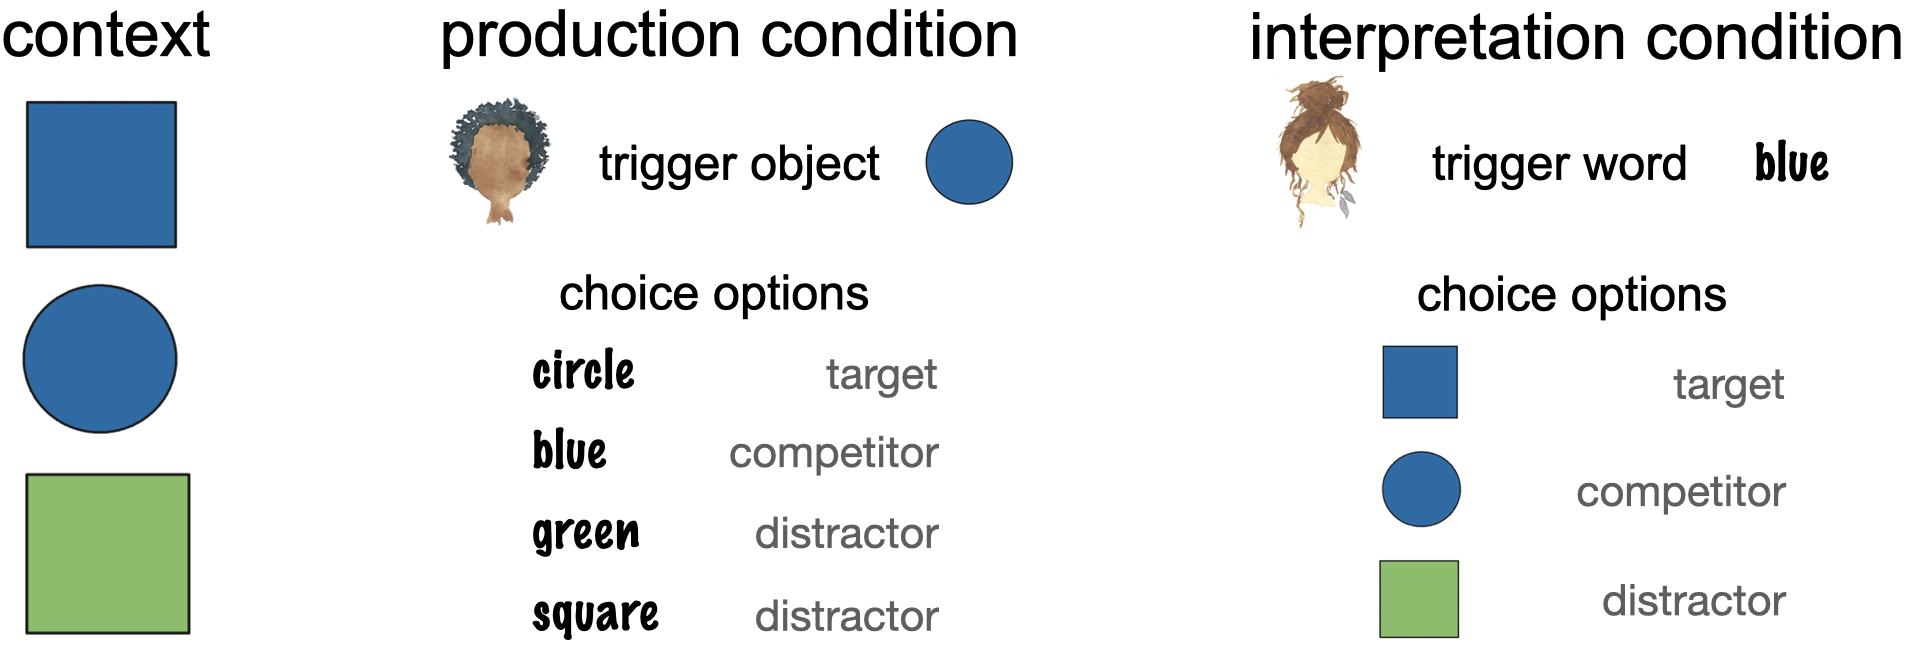
\includegraphics[width = 0.8\textwidth]{00-pics/reference-game.png}

  \caption{Structure of a reference game with human participants. Each trial consists of a set of objects, the so-called context. In production trials, participants choose a single word to describe a trigger object from the context. In interpretation trials, an object is selected as the likely object a trigger word referring to.}
  \label{fig:ref-game}
\end{figure}

Reference games are an established, well-understood and austere experimental paradigm to test human decision making in abstract communicative tasks \citep[e.g.,][]{FrankGoodman2012:Predicting-Prag,DegenFranke2013:Cost-Based-Prag,QingFranke2013:Variations-on-a,Frank2016:Rational-speech,SikosVenhuizen2021:Reevaluating-pr}.
A reference game consists of two players, a speaker and an interpreter, who jointly observe a set of objects, usually referred to as context (see Figure~\ref{fig:ref-game}).
In the \textbf{production condition}, the speaker is assigned a \emph{trigger object} from the context set which they have to describe to the interpreter.
In the \textbf{interpretation condition}, the interpreter observes a description, here called \emph{trigger word}, and chooses one of the objects from the context set.
The goal of the game is, for the speaker, to choose a description that enables the interpreter to choose the trigger object; and, for the interpreter, to guess correctly which object the speaker had in mind when using the trigger word.

The example in Figure~\ref{fig:ref-game} is a standard case, which we will use throughout, where human choices are informative about the pragmatic reasoning that human decision makers engage in.
In this example, there are two features that differ across three objects (here shape and color).
One object shares both its color and shape with one other object, while the two other objects have one unique feature (e.g., being the only circle, or the only green object).
%
In a critical production trial, the trigger object to describe is one of the two objects with a unique feature.
The speaker has four words to choose from.
The \textbf{target utterance} is the word which uniquely describes the trigger object.
The \textbf{distractor utterance} is the word that is true of the trigger object, but also true of another object.
The other utterances, both of which are false of the trigger object are \textbf{competitor utterance}.
%
In a critical interpretation trial, the trigger word is one that is true of two of the three objects.
If participants engage in pragmatic thought, they might reason that \emph{if} the speaker had wanted to refer to one of the two objects of which the trigger word is true (blue square and blue circle in Figure~\ref{fig:ref-game}), the speaker could have used a more informative word for exactly one of those two objects (``circle''), so they are more likely to refer to the \textbf{target object} (the blue square in Figure~\ref{fig:ref-game}).
The \textbf{competitor object} is the other object of which the trigger word is true.
The \textbf{distractor object} is the object of which the trigger word is false.

We replicated a simple reference game with human participants in which each trial instantiated the structure of the example shown in Figure~\ref{fig:ref-game}.
While previous reference games with human participants used pictorial representations of objects, and sometimes even pictorial representations of messages, we implemented a text-only version in order to be able to compare the predictions of LLMs for human data, when both LLMs and humans processed the same textual representation of the stimuli.
The experiment was realized as an online task using \texttt{magpie} \citep{FrankeJi:magpie:-Minimal}.\footnote{
  The code for the experiment can be found at \href{https://github.com/magpie-ea/magpie3-text-refgame}{https://github.com/magpie-ea/magpie3-text-refgame}, and a live version of the experiment can be tested at \href{https://magpie-ea.github.io/magpie3-text-refgame/}{https://magpie-ea.github.io/magpie3-text-refgame/}.
}


\subsection{Participants}
\label{participants}

A total of 302 participants were recruited via Prolific for monetary
compensation (\textsterling0.45, corresponding to roughly \textsterling 15.40 per hour).
All participants self-identified as native speakers of English.

\subsection{Materials \& design}
\label{materials-design}

We created 100 different items as stimulus material via a stochastic process.
Each item is a different textual description of a reference game with the same logical structure as the example from Figure~\ref{fig:ref-game}.
For each item, the context consisted of three objects.
As in the original paper by \citet{FrankGoodman2012:Predicting-Prag}, objects are defined by a triple of properties, namely a color, a shape and a texture.
For each property, there were four possible values, e.g., blue, green, red, and orange for color.
The sampled items differed in terms of the properties of the objects in the context set, and in terms of the order in which the objects and expression alternatives were presented in the text.
Figures~\ref{fig:refgame-screenshot-production} and \ref{fig:refgame-screenshot-interpretation} from Appendix~\ref{sec:scre-from-online} show example screenshots from the experiment.

\subsection{Procedure}
\label{procedure}

For each participant the experiment sampled four different items.
Participants first played two of these in the production condition, then the other two in the interpretation condition.


\subsection{Results}\label{results}

The overall distribution of choices that correspond to the target, competitor, and distractor states is shown in Figure~\ref{fig:refgame-counts}.\footnote{
  The production condition actually has two distractor choices.
  Here and in the following, these are lumped together as a single category, also when modeling random errors in later models.
  This is a simplification but does not change anything of substance.}
It is interesting that the distractor options were chosen rather often.
We also see that the number of target choices is higher in the production condition than in the interpretation condition.
This is in line with previous experimental results on human reference games.
% \citep{QingFranke2013:Variations-on-a}.
For example, in previous forced-choice reference games with human participants with pictorial presentations of objects, \citet{QingFranke2013:Variations-on-a} observed the following proportions of target, competitor and distractor options: $\tuple{0.882, 0.118, 0}$ in the production and $\tuple{0.492, 0.506, 0.003}$ in the interpretation condition (for 288 observations in each condition).

\begin{figure}[t]
  \centering

    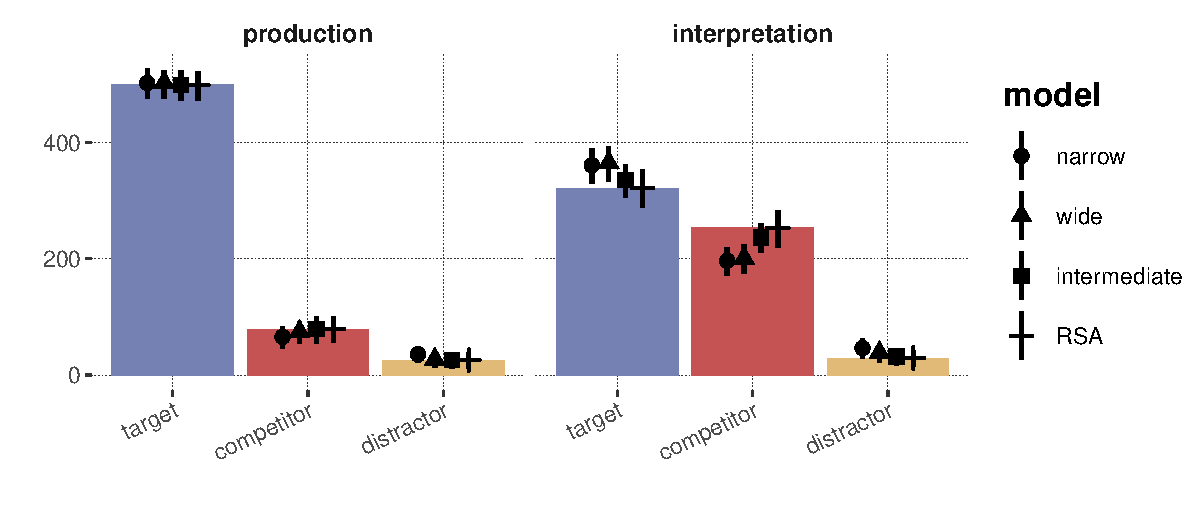
\includegraphics[width=0.9\linewidth]{00-pics/PPC-alpha-eps-model.pdf}

    \caption{Counts of choices from reference games with human participants (colored bars), with summary statistics from the posterior predictive distribution of four models (shapes and error bars).
      Shapes show the mean of the posterior predictive distributions of the RSA model and three further models derived from item-level LLM-supplied scores.
      Error-bars show corresponding 95\% credible intervals of the posterior predictive.
    }
  \label{fig:refgame-counts}
\end{figure}


%%%%%%%%%%%%%%%%%%%%%%%%%%%%%%%%%%%%%%%%%%%%%%%%%%
\section{Model predictions from probabilistic pragmatics}
\label{sec:model-pred-from}
%%%%%%%%%%%%%%%%%%%%%%%%%%%%%%%%%%%%%%%%%%%%%%%%%%

Data from reference games with human participants have been variously analyzed with probabilistic models using inspiration from behavioral game theory \citep[e.g.,][]{DegenFranke2013:Cost-Based-Prag}, probabilistic Bayesian modeling \citep[e.g.,][]{FrankGoodman2012:Predicting-Prag} or other forms of probabilistic modeling \citep[e.g.,][]{GattGompel2013:Are-we-Bayesian}.
Common to these approaches is that they derive or define, based on some explicit conceptual motivation, a parameterized stochastic speaker policy, $P_{S}(u \mid s; \theta_{S})$, modulated by parameters $\theta_{S}$, for a speaker's choice of expression or utterance $u$ given a referent or state $s$, which the speaker wants to communicate;
and a stochastic listener policy, $P_{L}(s \mid u; \theta_{L})$, capturing the probability of choosing a referent $s$ for utterance $u$.

As a concrete example, we introduce the Rational Speech Act (RSA) model first described in this form by \citet{FrankGoodman2012:Predicting-Prag} \citep[for overview see][]{FrankeJager2015:Probabilistic-p,GoodmanFrank2016:Pragmatic-Langu,StevensBenz2018:Game-Theoretic-,ScontrasTessler2021:A-practical-int,Degen2023:The-Rational-Sp}.
The RSA model defines pragmatic reasoning as a sequence of iterated (soft-)optmization of policies, grounding out in literal interpretation.
If $\mathfrak{L}(s,u) \mapsto \set{0,1}$ is a semantic meaning function mapping each pair of state $s$ and utterance $u$ to a (binary) truth-value, and if $P_{s}$ is a prior over states, a literal listener policy is defined as:
%
\begin{align*}
 P_{L_{0}}(s \mid u) \propto \mathfrak{L}(s,u) P(s)\,.
\end{align*}
%
The pragmatic speaker policy is defined as soft-optimizing the choice of utterance to minimize the literal listener's surprisal for the state to be communicated (e.g., the trigger object/nicefra):
%
\begin{align*}
  P_{S}(u_{i} \mid s, \alpha) & \propto \expo \left [ \log P_{L_{0}}(s \mid u_{i}) \right ] \,.
\end{align*}
%
Finally, the pragmatic listener is defined as the policy resulting from applying Bayes rule, solving the inverse-problem for the previously defined speaker policy:
%
\begin{align*}
  P_{L}(s \mid u, \alpha) \propto  P_{S}(u \mid s, \alpha) \  P(s) \,.
\end{align*}

\begin{figure}[t]
  \centering
  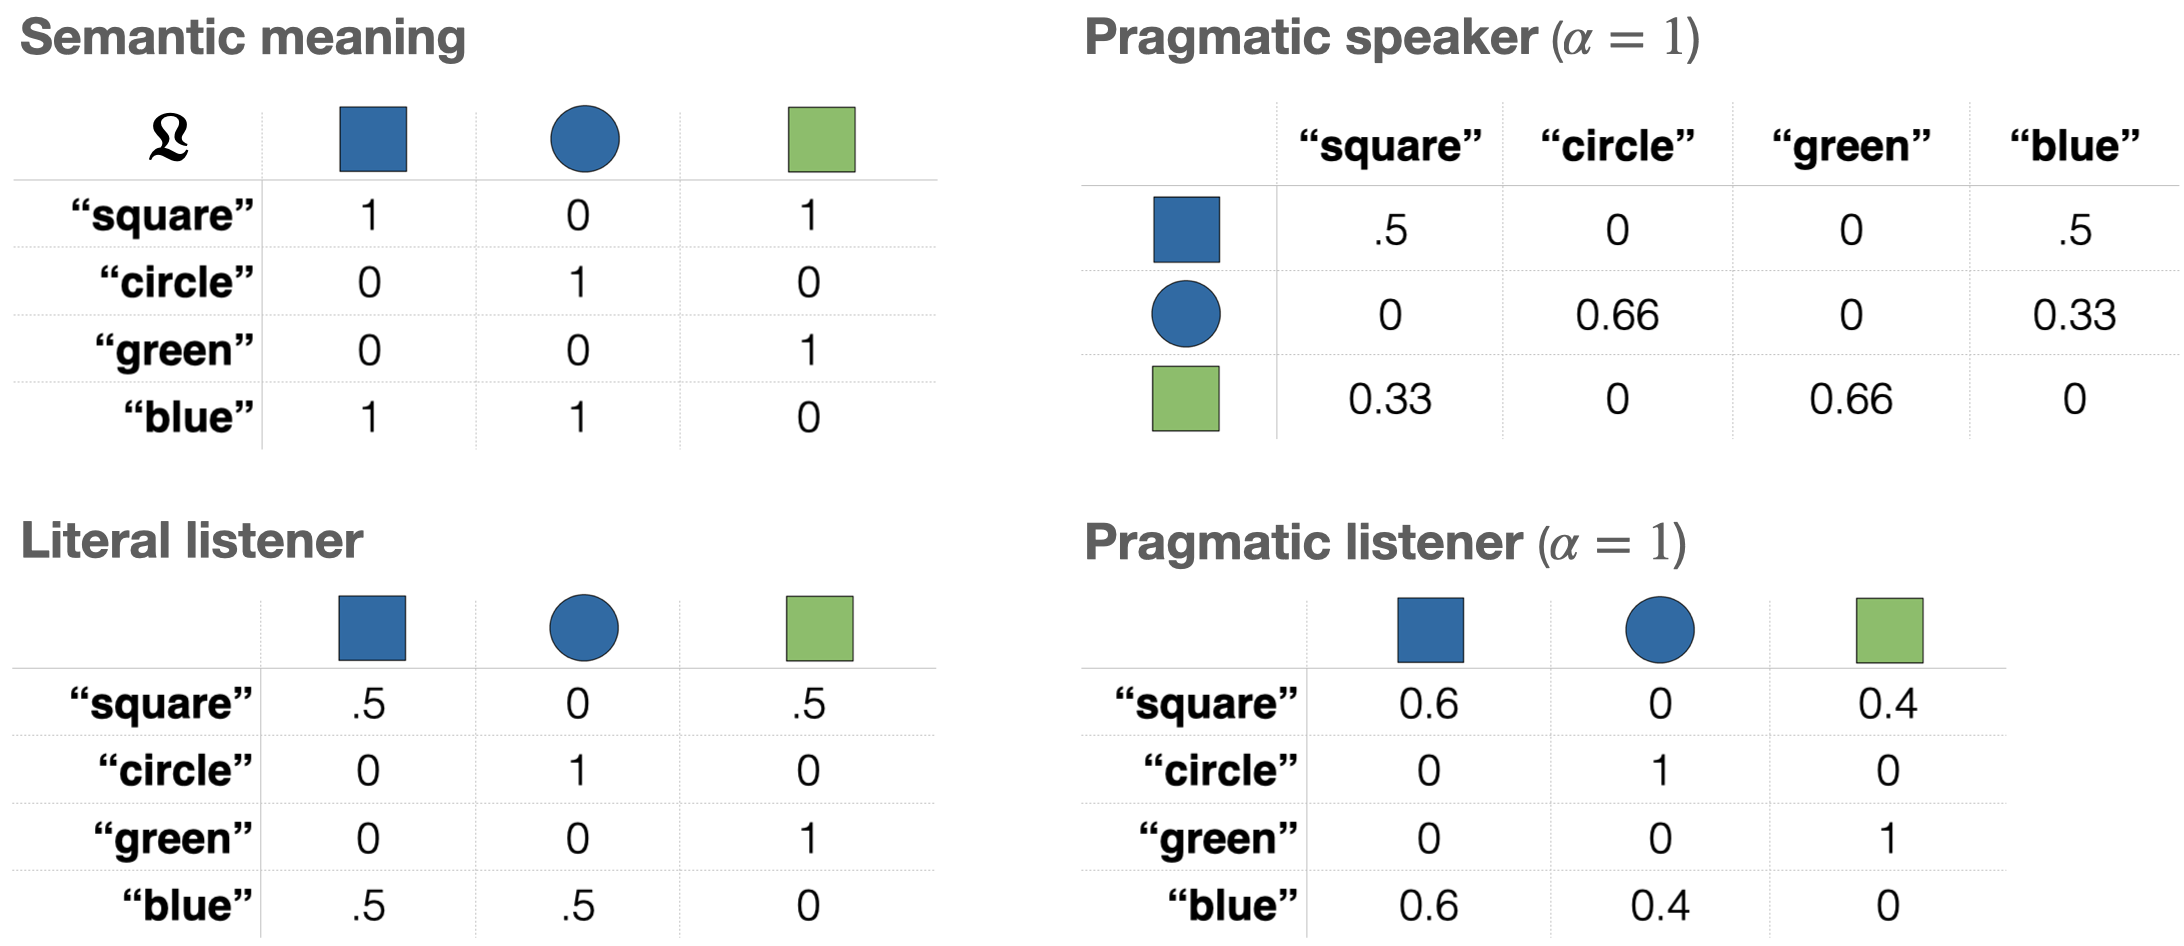
\includegraphics[width = 0.9 \textwidth]{00-pics/RSA-example.png}
  \caption{
    Example of predictions from the RSA model (with $\alpha=1$).
    The semantic meaning is shown as a matrix of binary truth-values.
    The policies of literal listener, pragmatic speaker and listener are calculated for uniform priors over state (referents) for $\alpha=1$ are shown as row-stochastic matrices.
  }
  \label{fig:RSA-example}
\end{figure}

Figure~\ref{fig:RSA-example} gives example calculations (assuming a flat prior $P(s)$ and $\alpha=1$) for the reference game from Figure~\ref{fig:ref-game}.
For $\alpha=1$, the model predicts that the probabilities of target, competitor and distractor options are $\tuple{\nicefrac{2}{3}, \nicefrac{1}{3}, 0}$ for the production, and $\tuple{\nicefrac{3}{5}, \nicefrac{2}{5}, 0}$ for the interpretation condition.
Increasing $\alpha$ will increase the odds of target over competitor choices.
Yet, the model also predicts probability zero for distractor choices, so that the human data shown in Figure~\ref{fig:refgame-counts}, where the distractor option was chosen in both conditions, would immediately rule out the model entirely.
It is therefore common to include a small error probability $\epsilon$, with which a choice would be made at random \citep[e.g.,][]{LeeWagenmakers2013:Bayesian-Cognit}: if $P_{r}(R_{l}, C, \alpha_{c})$ is the RSA model's probabilistic prediction for response category $R_{l}$ (target, competitor, or distractor) for condition $C$ (production or interpretation) and condition-specific optimality $\alpha_{c}$, the random-error smoothed prediction is:
\begin{align*}
  P_{r}(R_{l}, , C; \alpha_{c}, \epsilon_{c}) = (1 - \epsilon) \  P_{r}(R_{l}, C; \alpha_{c}) +  \nicefrac{\epsilon_{c}}{3}\,,
\end{align*}
where $\epsilon_{c}$ is a (condition-specific) parameter giving the probability that a choice was made by randomly guessing.\mf{FC objected to ``condition-specificity'' which is fair, but I leave it as it was; my reasoning: we use model checking to rule out models; in this setting the conservative strategy is to err on the side of making the models too powerful (even at the cost of conceptual plausibility)}
The result is a four-parameter model, one pair of parameters per condition, which provides a likelihood function for the categorical choice data and so can be fitted to the data and compared against other probabilistic models providing a likelihood function for the same data.

Parameterized predictions like $P_{r}(R_{l}, , C; \alpha_{c}, \epsilon_{c})$ can be assessed in the light of the empirical data with the usual tools of Bayesian data analysis \citep[e.g.][]{GelmanCarlin2014:Bayesian-Data-A,McElreath2016:Statistical-Ret,Lambert2018:A-Students-Guid}.
Let $\alpha_{c}\sim \text{log-Normal}(0.5,1)$ have a reasonably wide log-Normal prior, and let $\epsilon_{c} \sim \text{Beta}(1,5)$ have a Beta prior favoring small values.
Using Stan \citep{Team2023:The-Stan-Core-L} for Bayesian inference, we obtain estimates of posterior credible values of model parameters (summary statistics of which are shown in Table~\ref{fig:posterior-stats}).
\mf{include information on MCMC, samples, warm-up etc.; follow Kruschke recipe}


To assess goodness-of-fit, we can use the \emph{posterior predictive distribution}, i.e., the model's predictions about data of the same size and structure as the training data.
\mf{maybe insert formal definition of post-pred distribution?}
As a minimal bar, we would require a model trained on observed data $D_{\text{obs}}$ to not be surprised by $D_{\text{obs}}$.
Figure~\ref{fig:refgame-counts} shows summary statistics (means and 95\% credible intervals) for the posterior predictive distribution of the RSA model (among other models to be introduced later).
We see that the RSA model passes this ``visual posterior predictive check'' \citep{Kruschke2011:Doing-Bayesian-} for both conditions.
To corroborate the visual impression, Table~\ref{tab:Bppp-values} shows sample-based estimates of Bayesian posterior predictive $p$-values, using likelihood of the observed data as a test statistics.
These values approximate the probability that a model trained on $D_{\text{obs}}$ would predict future data of the same size and format that is at least as unlikely as the data $D_{\text{obs}}$ itself.
% Low values therefore indicate that the trained model would be highly surprised by the data it was trained on; an indication that it failed to capture something essential about the training data.
% The results from Table~\ref{tab:Bppp-values} show that the RSA model passes this numerical test of model adequacy.

The following sections apply these tests of Bayesian model criticism also to models built around predictor values from LLMs.
Section~\ref{sec:item-level-pred} first looks at the data from each item individually, before Section~\ref{llm-predictions-for-reference-games} investigates different ways for deriving condition-level predictions.


%%%%%%%%%%%%%%%%%%%%%%%%%%%%%%%%%%%%%%%%%%%%%%%%%%
\section{Item-level predictions from LLMs}
\label{sec:item-level-pred}
%%%%%%%%%%%%%%%%%%%%%%%%%%%%%%%%%%%%%%%%%%%%%%%%%%

Figure~\ref{fig:refgame-counts} shows the condition-level counts for human choices for all of the 100 different items combined.
An LLM, on the other hand, first and foremost makes predictions about each item.
As mentioned previously, the items of the reference game experiment differ in the task-relevant features (color, shape, texture), as well as the order of presentation of states and words.
We expect both human and LLM predictions to vary between different items: e.g., humans seem to have preferences for some features \citep{QingFranke2013:Variations-on-a}, maybe even leading to over-production of informationally irrelevant material \citep{DegenHawkins2020:When-redundancy} \mf{more refs on (color) over-specification}; and machines may be susceptible to the presentation of the order of choice options. \mf{@PT references from the NLP literature on effects of prompt variation?}
The main question to be addressed in this section is whether a standard item-level score from LLMs provides a good fit, if we aim at predicting the human data separately for each item, not as a condition-level average.

For a set-up in which the task descriptions and choice options are all text-based, predictions of LLMs at the item-level can be derived as a function of the (log) probabilities assigned to the continuations corresponding to each choice option after processing the task description.
Let $C$ be the experimental condition of interest (here: the production or interpretation condition).
Let \(\set{I_1, \dots I_m}\) be the multi-set of items that occurred in the human experiment for condition $C$.\footnote{
  By using a multi-set, which may contain a single task multiple times, we produce aggregate predictions for exactly the set of item that the participant group saw, which provides the most fitting counterpart to the human data.
}
Each item $I_{k}$ consists of a task description $T_{k}$ and $l$ choice options $O_{k1}, \dots, O_{kl}$, which are treated as textual continuations of the task description (see Appendix~\ref{sec:examples-items-llm} for an example).
For each item $I_{k}$, let $F(R_{l}, I_{k})$ be the choice option $O_{ki}$ that corresponds to \emph{response type} $R_{l}$ (here: target, competitor, distractor).\footnote{In the current set-up the response type ``distractor'' has two instantiations in the production condition. Since choice options are a single word in the production condition, for simplicity, we lump both of the distractor words together and treat them as a single option by taking the sum of the log-probabilities for both distractor words.}
The \emph{item-level score} $S(O_{{ki}}, I_{k})$ for option $O_{ki} = w_{ki1}, \dots w_{kin}$ of item $I_{k}$ is defined as the log-probability of continuation $O_{ki}$ after prompt $T_{k}$:\footnote{Numerically, we worked with \emph{average} log-probabilities. As in our experiment, all choice options had the same number of words, this is largely irrelevant, except for the effect of the $\alpha$ parameter in the interpretation condition. Using length-corrected log-probabilities is the same as using raw log-probabilities with an $\alpha$ parameter divided by the number of words. In this way, we make the $\alpha$ parameter more meaningfully comparable across conditions.}
%
\begin{align*}
S(O_{ki}, I_{k}) =  \sum_{j=1}^n \log P_{\text{LLM}} \left(w_{kij} \mid T_{k}, w_{ki1}, \dots, w_{ki(j-1)} \right)  \,.
\end{align*}
%
\mf{check if formula is redundant; already introduced?}
The item-level score of response type $R_{l}$ is $S(R_{l}, I_{k}) = S(F(R_{l}, I_{k}))$.

Using item-level scores from GPT-3.5, we fit a model to the human data at the item-level \mf{which model exactly, when assessed, cite paper}.
The data to be explained is the set of all triples of response type counts $\tuple{t_{k}, c_{k}, d_{k}}$ (target, competitor, distractor), separately for each item $I_{k}$.
The model's predictions for the data from item $I_{k}$ from condition $C$ (production or interpretation) are:
%
\begin{align*}
  P_{\text{item}}(R_{l}, C, I_{k}, \alpha_{c}, \epsilon_{c}) \propto \frac{\expo \left( \alpha_{c} \ S(R_{l}, I_{k}) \right )}{ \sum_{l'} \expo \left( \alpha_{c} \ S(R_{l'}, I_{k}) \right )} + \epsilon_{c}\,.
\end{align*}
%
In words, we use a single pair of parameters $\alpha_{c}$ and $\epsilon_{c}$, one for each condition, take the LLM's item-level scores for each item, and derive the response probabilities in the exact same way as before.
% Notice that item-level scores are the same for all three types of models introduced and compared in the previous section, so that this by-item analysis applies to the raw LLM prediction irrespective of down-stream aggregation.
Priors on parameters are as for the RSA model described in Section~\ref{sec:model-pred-from}.

\begin{figure}[t]
  \centering

  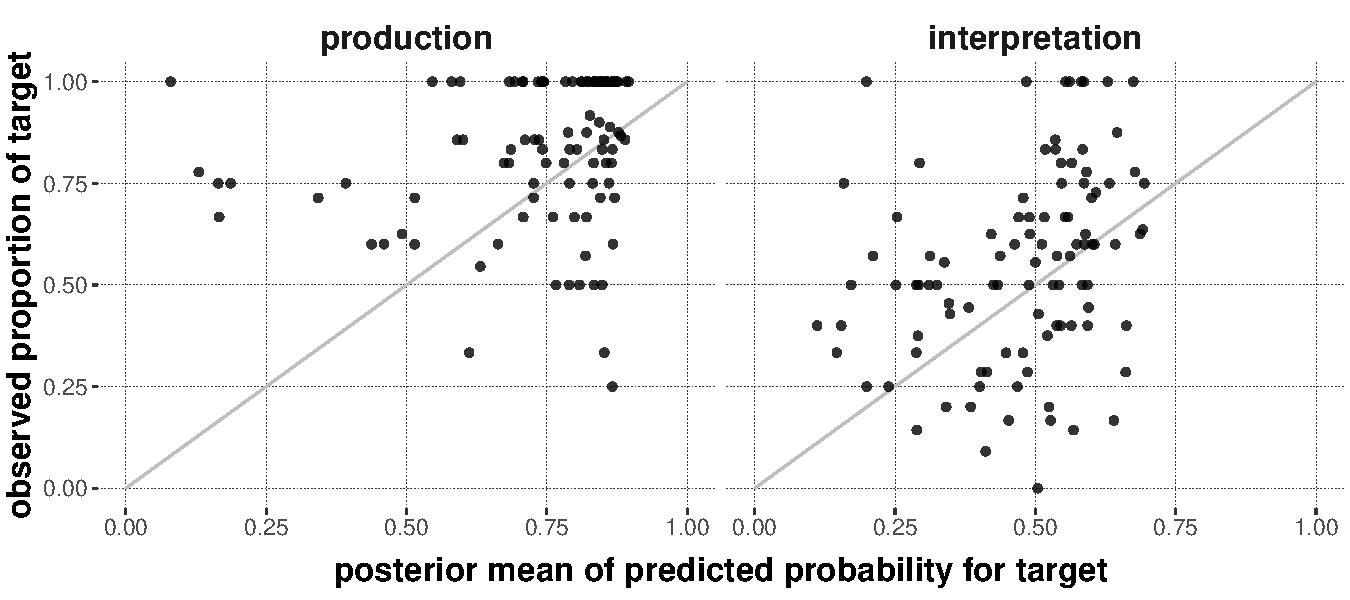
\includegraphics[width = 0.9\linewidth]{00-pics/item-combined-obs-pred.pdf}

  \caption{
    Item-level prediction-observation plot.
    Each dot represents an item.
    The $x$-coordinate represents the mean of the posterior prediction for the target choice probability for the given item.
    The $y$-coordinate represents the observed proportion of target choices for that item.
    The gray line (identity function) is the ideal prediction.
  }
  \label{fig:item-level-obs-pred}
\end{figure}

Figure~\ref{fig:item-level-obs-pred} shows that the item-level LLM scores predict variance which is not borne out by the human data.
Concretely, the plot shows, for each item, mean posterior estimates of the model's predicted probability of choosing the target option ($x$-axis), together with the observed proportion of target choices in the human data ($y$-axis).
There is ample variation in the model's predictions, especially visible in the production condition, owing to the fact that the item-level scores of the LLM sometimes clearly favor another option than the target choice.
So, the model itself predicts systematic variability at the item level.
The human data, too, show variability at the item-level, but there is no (visual) indication that the item-level variability predicted by the LLMs is borne out by the human data.

Sampling-based approximations of Bayesian posterior predictive $p$-values for the by-item analysis are very low (0.0001 for production, 0 for interpretation), suggesting that the unaggregated item-level LLM predictions are inadequate predictors of the human data.
In contrast, using the global, item-independent RSA model predictions to fit the item-level data, we obtain estimates of posterior predictive $p$-values that do not discredit the model ($0.338$ for production, $0.252$ for interpretation).
These results suggest that LLM-based probabilistic predictions may imply item-level variance that is not attested in the human data.
Put more strongly, a model that seeks to predict what human participants choose on a by-item level, based on the most obvious item-level score, is ruled out by experimental data.



%%%%%%%%%%%%%%%%%%%%%%%%%%%%%%%%%%%%%%%%%%%%%%%%%%
\section{Condition-level predictions}
\label{llm-predictions-for-reference-games}
%%%%%%%%%%%%%%%%%%%%%%%%%%%%%%%%%%%%%%%%%%%%%%%%%%

This section explores different ways of deriving a probabilistic likelihood function for the human data from an LLM at the aggregate, condition-level.
Using log-probabilities for each answer option as a basic item-level score, there are at least three conceivable ways of deriving condition-level predictions by averaging over item-level variation (see Figure~\ref{fig:measures-overview}).
In the following, we first describe the different options of deriving LLM-based predictors.
We then compare all probabilistic models based on their adequacy of explaining the human choice data.

\begin{figure}
  \centering
  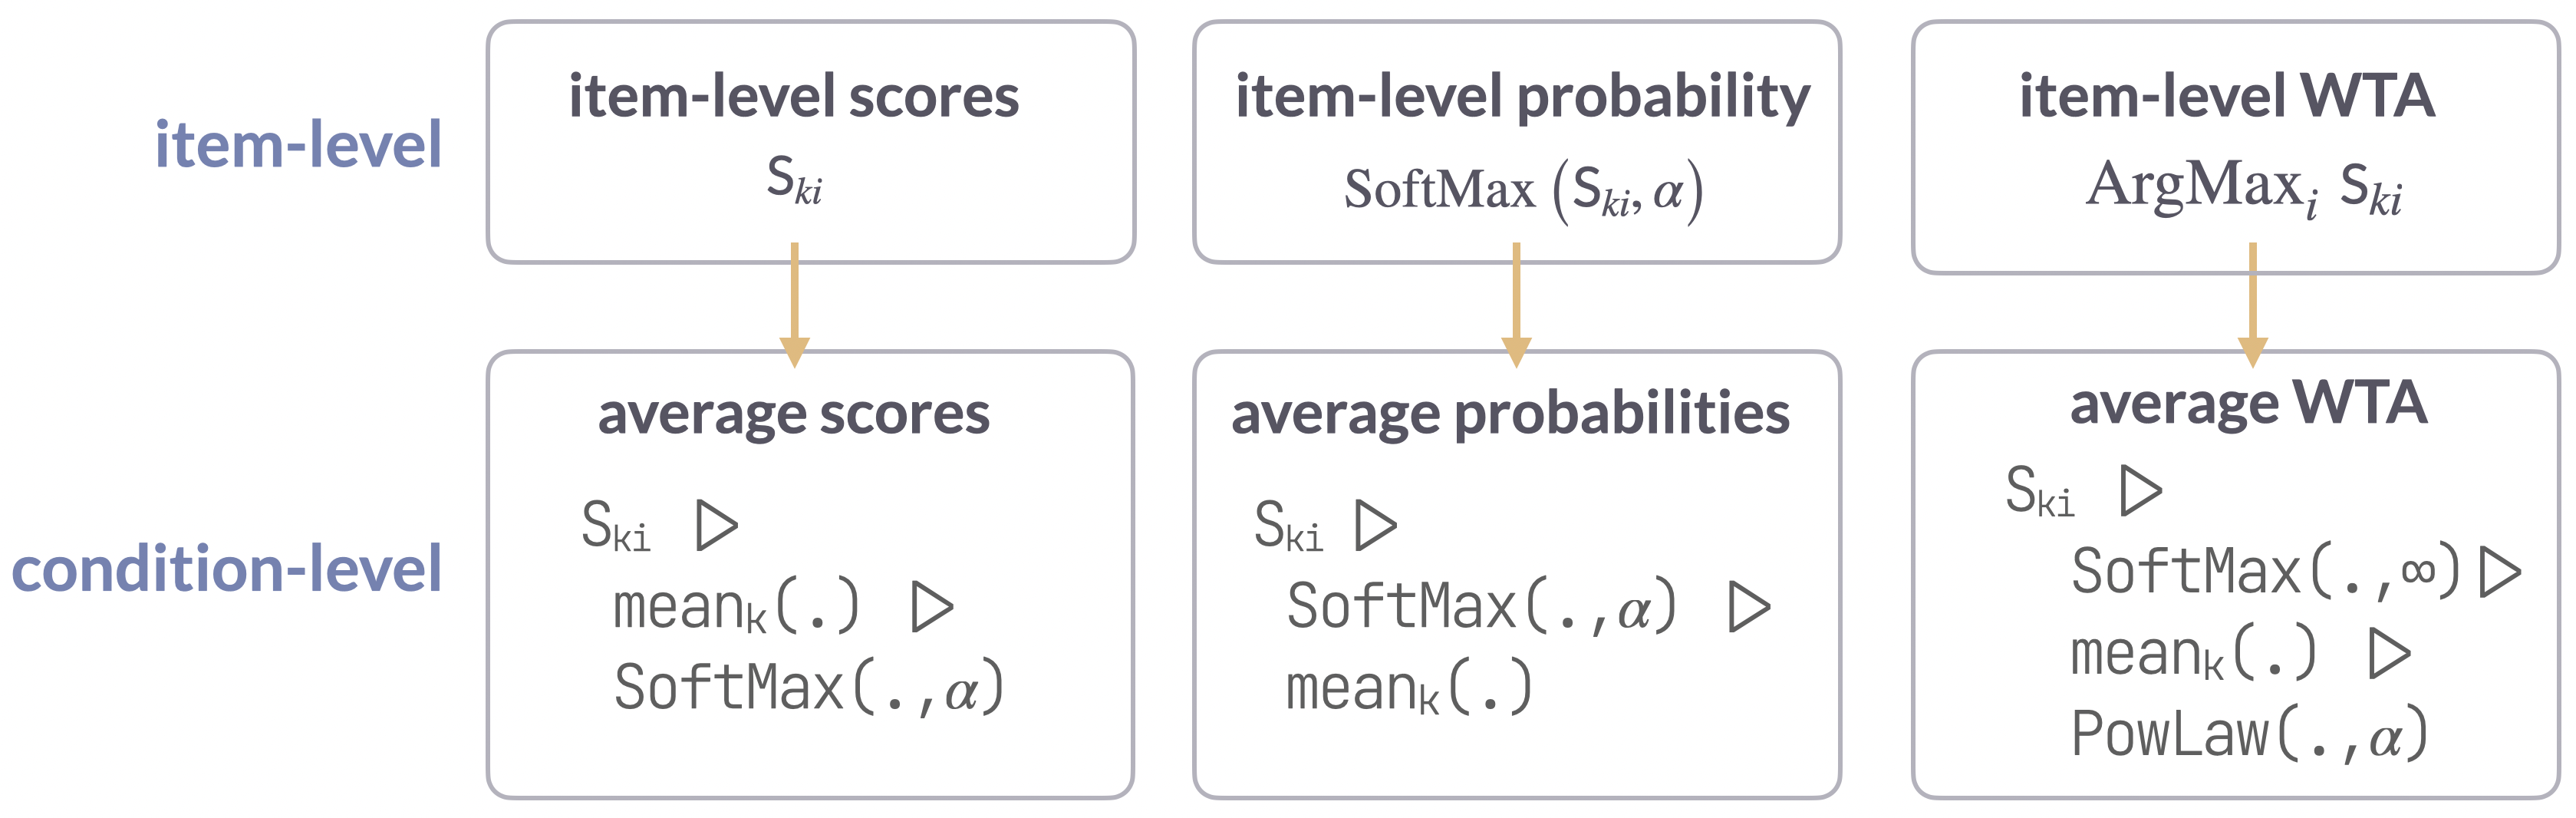
\includegraphics[width=0.9\textwidth]{00-pics/measures-overview.png}
  \caption{
    Schematic overview over three different approaches of obtaining condition-level predictions by aggregating over item-level scores.
    The basic item-level score is average next-word log probability.
    This can be taken as-is into averaging (narrow-scope aggregation), or first transformed from log- into probability-space, either with optimization before (wide scope) or after averaging (intermediate scope).
    The notation for the condition-level options uses pseudo-code to more clearly reflect the relevant operator scope differences (where triangles represent the pipe operator).
  }
  \label{fig:measures-overview}
\end{figure}

Condition-level predictions are a probability distribution over response types, obtained from item-level scores $S(R_{l}, I_{k})$ by averaging over all items belonging to the relevant condition.
To map non-normalized scores $\myvec{s} = \tuple{s_{1}, \dots, s_{l}}$ to probabilities $\myvec{p} = \tuple{p_{1}, \dots, p_{l}}$ with different degrees of optimization, a common choice is the softmax function with optimality parameter $\alpha$:
%
\begin{align*}
 \text{SoftMax}(\myvec{s}, \alpha) = \myvec{p}, \text{where } p_{i} \propto \expo \left (\alpha p_{i} \right )\,.
\end{align*}
%
The softmax function can furthermore be decomposed into a first step of mapping scores to probabilities, and subsequently reweighing probabilities via a power-law transformation \citep[c.f.,][]{FrankeDegen2023:The-softmax-fun}:
%
\begin{align*}
  \text{SoftMax}(\myvec{s}, \alpha) & = \text{Pow}( \text{SoftMax}(\myvec{s}, 1) ; \alpha) \\
  \text{Pow}(\myvec{p} ; \alpha) & = \myvec{q}, \text{where } q_{i} \propto p_{i}^{\alpha}
\end{align*}
%
This means that there are three conceivable scope-sites for aggregating item-level information as shown in Figure~\ref{fig:measures-overview}.
Narrow-scope aggregation first aggregates the item-level scores, and then transposes the averages into (scaled) probabilities:
%
\begin{align*}
  % & \textbf{narrow-scope aggregation} \\
  & P_{n}(R_{l}, C ; \alpha) \propto \expo \left [  \alpha \ \frac{1}{m} \ \sum_{i = k}^{m} S(R_{l}, I_{k})  \right ]
    \tag*{\textcolor{gray}{[narrow-scope aggregation]}}
\end{align*}
%
Wide-scope aggregation, first transposes scores into probabilities, scales them and only aggregates over items last.
\begin{align*}
  % & \textbf{wide-scope aggregation} \\
  & P_{w}(R_{l}, C ; \alpha) \propto \frac{1}{m} \ \sum_{i = k}^{m} \frac{\expo \left( \alpha \ S(R_{l}, I_{k}) \right )}{ \sum_{l'} \expo \left( \alpha \ S(R_{l'}, I_{k}) \right )}
    \tag*{\textcolor{gray}{[wide-scope aggregation]}}
\end{align*}
%
Intermediate-scope aggregation performs item-level averaging after mapping scores onto probabilities (using softmax with $\alpha=1$), but before scaling (with a power-law transformation with variable $\alpha$):
\begin{align*}
  % & \textbf{intermediate-scope aggregation} \\
  & P_{i}(R_{l}, C ; \alpha) \propto  \left [ \frac{1}{m} \ \sum_{i = k}^{m} \frac{\expo \left( S(R_{l}, I_{k}) \right )}{ \sum_{l'} \expo \left( S(R_{l'}, I_{k}) \right )} \right ]^{\alpha}
    \tag*{\textcolor{gray}{[intermediate-scope aggregation]}}
\end{align*}

All three condition-level predictors coincide when there is only one item, of course.
For more items, wide-scope and intermediate-scope aggregation coincide when $\alpha = 1$.
In all other cases, the predictors are not guaranteed to be identical.
Conceptually, the main difference is what each measure considers to be the basic item-level unit to aggregate over.
Narrow-scope aggregation considers raw scores, which are \emph{not} probabilistic predictions at the item level.
Wide-scope aggregation considers $\alpha$-optimized probabilities at the item level, which is compatible with a procedure of sampling, via softmax decoding, item-level answer options.
Wide-scope aggregation contains the ``winner-takes-all'' procedure for accuracy scoring in common benchmark tests for $\alpha \rightarrow \infty$.
Finally, like wide-scope aggregation, intermediate-scope aggregation is also compatible with a sampling based picture, but would use pure decoding (without $\alpha$-optimization) at the item level and reserves the scaling of probability distributions to a stage \emph{after} aggregation.

\begin{table}[t]
  \centering

  % 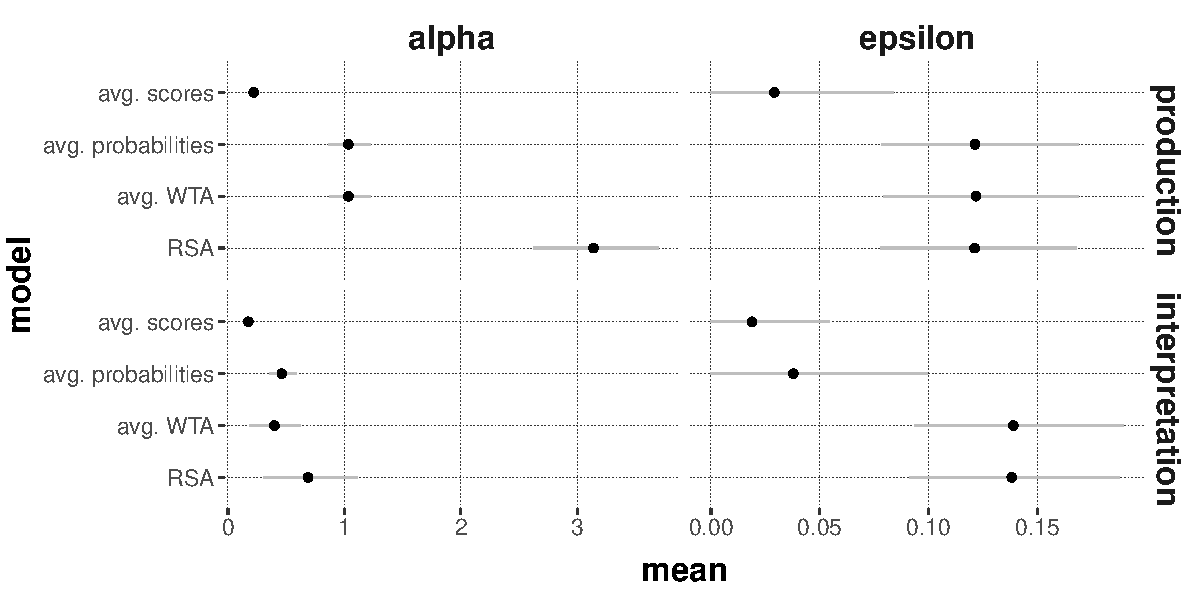
\includegraphics[width=0.9\linewidth]{00-pics/posterior-stats.pdf}

  \begin{tabular}{llllcr}
    \toprule \addlinespace[1ex]
    model        & condition      & Parameter  & $|$95\% & mean & 95\%$|$ \\
    \midrule  \addlinespace[1ex]
    narrow       & production     & $\alpha$   & 0.19    & 0.22 & 0.26 \\
                 &                & $\epsilon$ & 0.00    & 0.04 & 0.11 \\
                 & interpretation & $\alpha$   & 0.15    & 0.18 & 0.20 \\
                 &                & $\epsilon$ & 0.00    & 0.02 & 0.06 \\ \addlinespace[0.75ex]
    intermediate & production     & $\alpha$   & 0.86    & 1.04 & 1.22 \\
                 &                & $\epsilon$ & 0.08    & 0.13 & 0.18 \\
                 & interpretation & $\alpha$   & 0.36    & 0.48 & 0.60 \\
                 &                & $\epsilon$ & 0.00    & 0.05 & 0.12 \\ \addlinespace[0.75ex]
    wide         & production     & $\alpha$   & 0.22    & 2.69 & 8.79 \\
                 &                & $\epsilon$ & 0.08    & 0.13 & 0.19 \\
                 & interpretation & $\alpha$   & 0.19    & 1.08 & 6.03 \\
                 &                & $\epsilon$ & 0.00    & 0.06 & 0.18 \\ \addlinespace[0.75ex]
    RSA          & production     & $\alpha$   & 2.59    & 3.16 & 3.71 \\
                 &                & $\epsilon$ & 0.08    & 0.13 & 0.18 \\
                 & interpretation & $\alpha$   & 0.24    & 0.66 & 1.07 \\
                 &                & $\epsilon$ & 0.10    & 0.15 & 0.20 \\ \addlinespace[0.25ex]
    \bottomrule \\
  \end{tabular}

  \caption{
    Summary statistics of posterior samples.
    Number indicate estimates for lower and upper bounds of 95\% credible intervals and the posterior means.
    \mf{make wide format}
  }
  \label{fig:posterior-stats}
\end{table}

The three condition-level predictions yield three different probabilistic models, each with two pairs of condition-dependent parameters $\alpha_{c}$, and $\epsilon_{c}$.
Using priors and Bayesian posterior estimation as previously described for the RSA (see Section~\ref{sec:model-pred-from}), we obtain samples from the posterior over parameters and samples from the posterior predictive distributions.
The usual Bayesian summary statistics for posteriors over model parameters are shown in Table~\ref{fig:posterior-stats}.
What is noteworthy about these estimates is that the $\alpha_{c}$ parameters for the wide-scope model have a very large credible range.
This is because, already for values of $\alpha_{c} = 1$, the item-level predictions are virtually ``winner-takes-all'' choices, selecting the option with the maximum score with probability almost 1 for almost all items.
This implies that, by studying the posterior predictive distribution of the wide-scope model, we are virtually testing condition-level predictions from the standard WTA-strategy used for benchmark testing (see Section~\ref{motivation}).

Figure~\ref{fig:refgame-counts} shows the summary statistics (means and 95\% credible intervals) for each model's posterior predictive distribution.
We find that only the theoretical model (RSA) and the intermediate-scope model passes this ``visual posterior predictive check'' for both conditions; the other two models both overpredict the target choice rate and underpredict the competitor choice rate in the interpretation condition.
To corroborate the visual impression, Table~\ref{tab:Bppp-values} shows sample-based estimates of Bayesian posterior predictive $p$-values, using likelihood of the observed data as a test statistics.
Consequently, the results from Table~\ref{tab:Bppp-values} suggest that the narrow-scope model fails on the interpretation data, and is at most borderline compatible with the production data; that the wide-scope model is able to reproduce the production data, but fails on the interpretation data; and that only the intermediate-scope model is able to fully recover the data from both conditions.

\begin{table}[ht]
\centering

% \begin{tabular}{lrr}
%   \toprule
%   model        & production & interpretation \\ \midrule
%   narrow       & 0.05       & 0.00 \\
%   wide         & 0.51       & 0.00 \\
%   intermediate & 0.49       & 0.26 \\
%   RSA          & 0.49       & 0.52 \\
%   \bottomrule \\
% \end{tabular}

\begin{tabular}{lrrrr}
  \toprule
  & narrow & wide & intermediate & RSA \\ \midrule
  production & 0.05 & 0.51 & 0.49 & 0.49 \\
  interpretation & 0.00 & 0.00 & 0.26 & 0.52 \\ \bottomrule \\
\end{tabular}


\caption{Sample-based estimates of Bayesian posterior predictive $p$-values for each model and each condition, based on likelihood of the observed data as test statistic.}
\label{tab:Bppp-values}
\end{table}

These results tell us that not all ways of deriving condition-level predictions by averaging over item-level variation are equally good.
Some approaches clearly fail basic checks for statistical goodness-of-fit.
On the positive side, we also find that there is at least one model with predictors based on LLM-measures, namely the intermediate-scope model, which is able to recover the patterns in the data.
In other words, there is a way of deriving predictor values for condition-level forced-choice probabilities from an LLM such that, when fed into a common linking function (here with parameters $\alpha$ for optimization and $\epsilon$ for random error), the human choice probability can be reconstructed faithfully in its entirety.\footnote{
  A potential worry is that the intermediate-scope model is trivial in the sense that it could have predicted \emph{any} data observation.
  Appendix~\ref{sec:range-prior-pred} shows that this is not the case.
}
This implies that using LLM predictors for probabilistic predictions, such as in a neuro-symbolic model, might be possible if embedded in the proper link functions and if item-level variation is averaged out in the right way.


%%%%%%%%%%%%%%%%%%%%%%%%%%%%%%%%%%%%%%%%%%%%%%%%%%
\section{Conclusion}
\label{conclusion}
%%%%%%%%%%%%%%%%%%%%%%%%%%%%%%%%%%%%%%%%%%%%%%%%%%

It is not entirely ludicrous to use numerical predictions from LLMs are
part of predictive probabilistic models. But we have to be careful.
Ideally, we average out over low-level variation, such as from order of
presentation or similar ``nuisance,'' at least as long as we do not
understand what causes this variation in the predictions of models and
further research that investigates when exactly this variation accords
with empirically observed patterns.

This also implies that we should likely \emph{not} (yet) aspire to use
LLMs are models or individual- or item-level predictors.

( {TODO: rethink conclusion})

{to be continued}

\newpage
\appendix


%%%%%%%%%%%%%%%%%%%%%%%%%%%%%%%%%%%%%%%%%%%%%%%%%%
\section{Screenshots from the online experiment with human participants}
\label{sec:scre-from-online}
%%%%%%%%%%%%%%%%%%%%%%%%%%%%%%%%%%%%%%%%%%%%%%%%%%

Figure~\ref{fig:refgame-screenshot-production} shows a trial from the production condition, Figure~\ref{fig:refgame-screenshot-interpretation} one for the interpretation condition of the online experiment.

\begin{figure}[H]
  \centering
  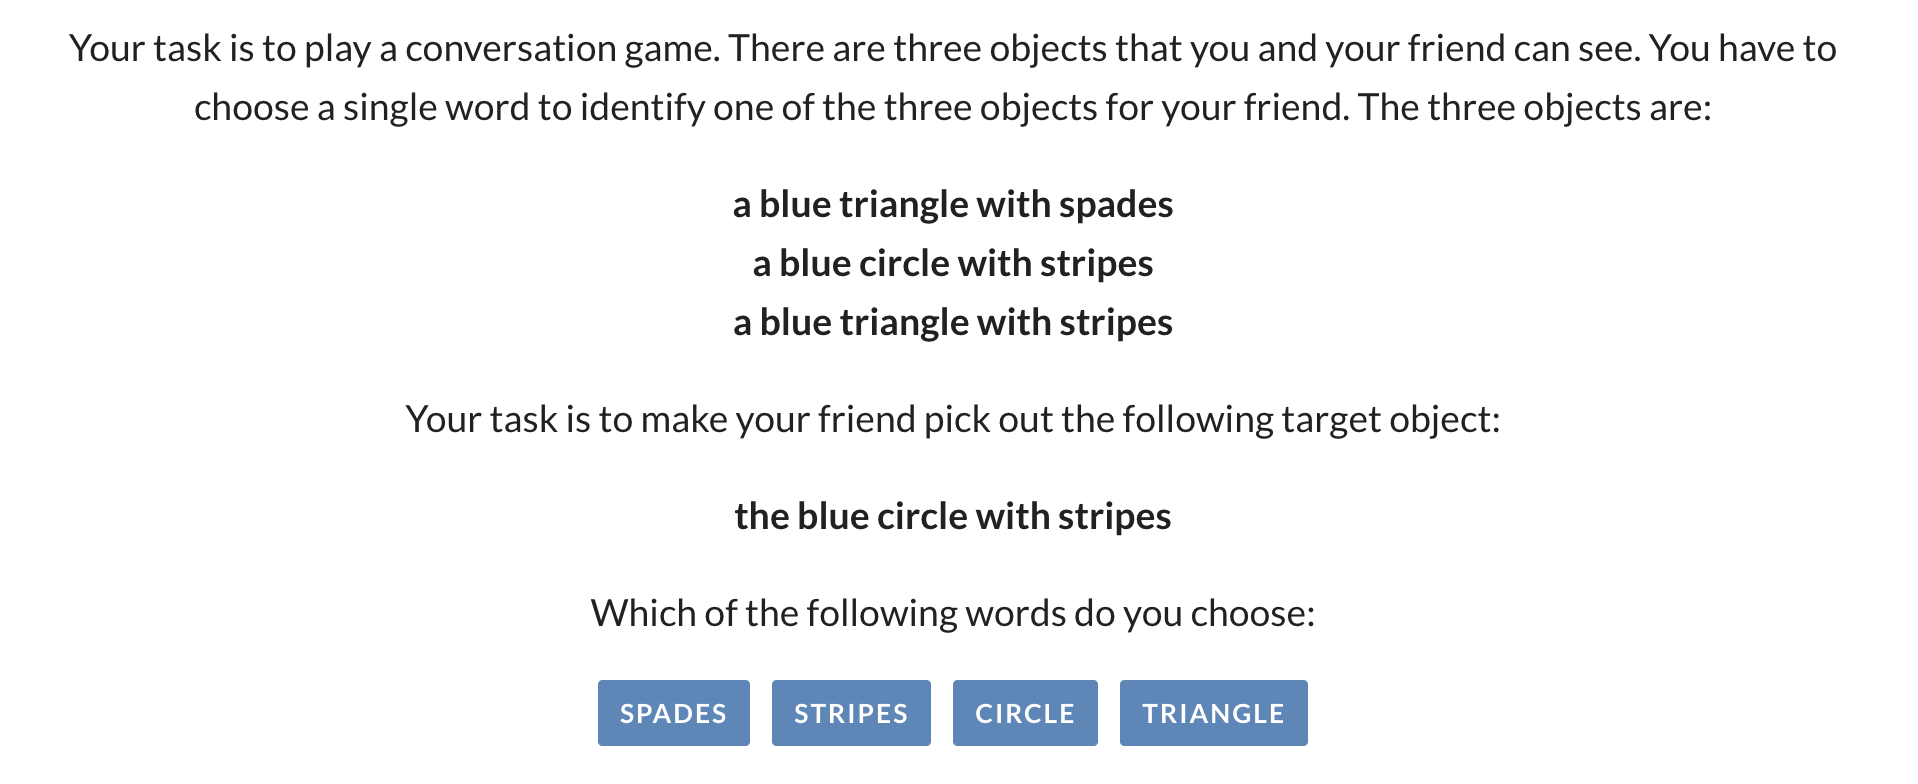
\includegraphics[width = 0.8\textwidth]{00-pics/refgame-production.png}

  \caption{Screen shot from a production trial of the online experiment.}
  \label{fig:refgame-screenshot-production}
\end{figure}

\begin{figure}[H]
  \centering
  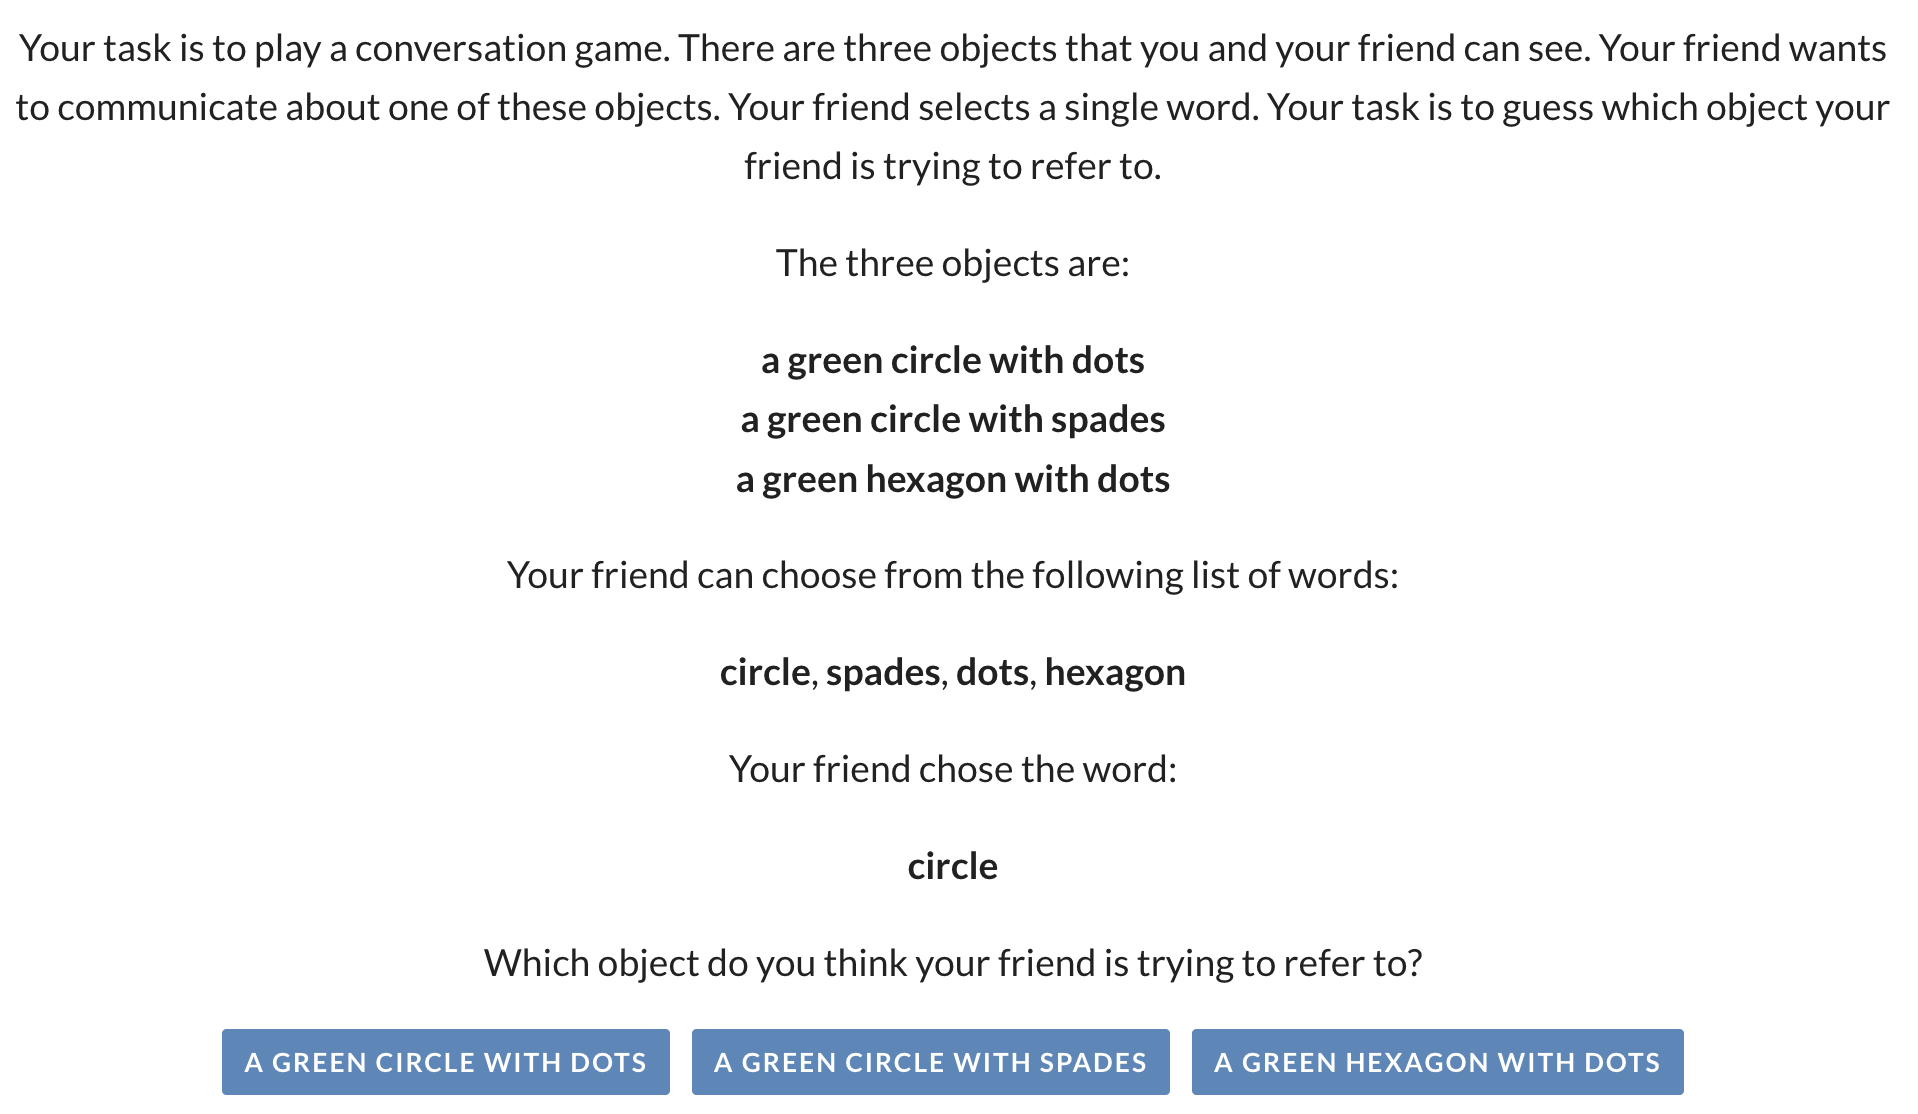
\includegraphics[width = 0.8\textwidth]{00-pics/refgame-interpretation.png}

  \caption{Screen shot from an interpretation trial of the online experiment.}
  \label{fig:refgame-screenshot-interpretation}
\end{figure}

\section{Example item for the LLM experiment}
\label{sec:examples-items-llm}

The text-based input for the LLM predictions mirrors the text in the human experiment, except that the LLM input also lists the set of all available choice options (which for the human experiment is unnecessary since this information is given by the buttons for the forced-choice selection).
For example, the task description $T_{k}$ for the item that corresponds to the production trial shown in Figure~\ref{fig:refgame-screenshot-production} is shown below (the actual input has no line breaks in the first paragraph):

\begin{verbatim}
Your task is to play a conversation game. There are three objects that
you and your friend can see. You have to choose a single word to identify
one of the three objects for your friend.

The three objects are:

a blue triangle with spades
a blue circle with stripes
a blue triangle with stripes

Your task is to make your friend pick out the following target object:

the blue circle with stripes

Which of the following words would you choose:

spades
stripes
circle
triangle

Your answer:

I would choose the word
\end{verbatim}


%%%%%%%%%%%%%%%%%%%%%%%%%%%%%%%%%%%%%%%%%%%%%%%%%%
\section{Range of prior predictions of intermediate-scope model}
\label{sec:range-prior-pred}
%%%%%%%%%%%%%%%%%%%%%%%%%%%%%%%%%%%%%%%%%%%%%%%%%%

It may seem that, given the freedom to adjust optimization $\alpha$ and random guessing rate $\epsilon$, some models might be able to explain \emph{any} data observation.
The intermediate-scope model, which was not discredited by model criticism in terms of recovery-based posterior predictive checks, is not trivial in this sense.
Figure~\ref{fig:prediction-range} shows the range of predictions that the intermediate-scope model is, in principle, capable of making (for the whole possible range of \(\alpha\) and \(\epsilon\) values, disregarding Bayesian priors).
There are distributions over response types which the model does not predict \emph{ex ante}.
For example, the model does not predict cases where the number of competitor choices is almost as high as the number of target choice, as would be the case if participants would consistently \emph{not} engage in pragmatic reasoning.


\begin{figure}[t]
  \centering

  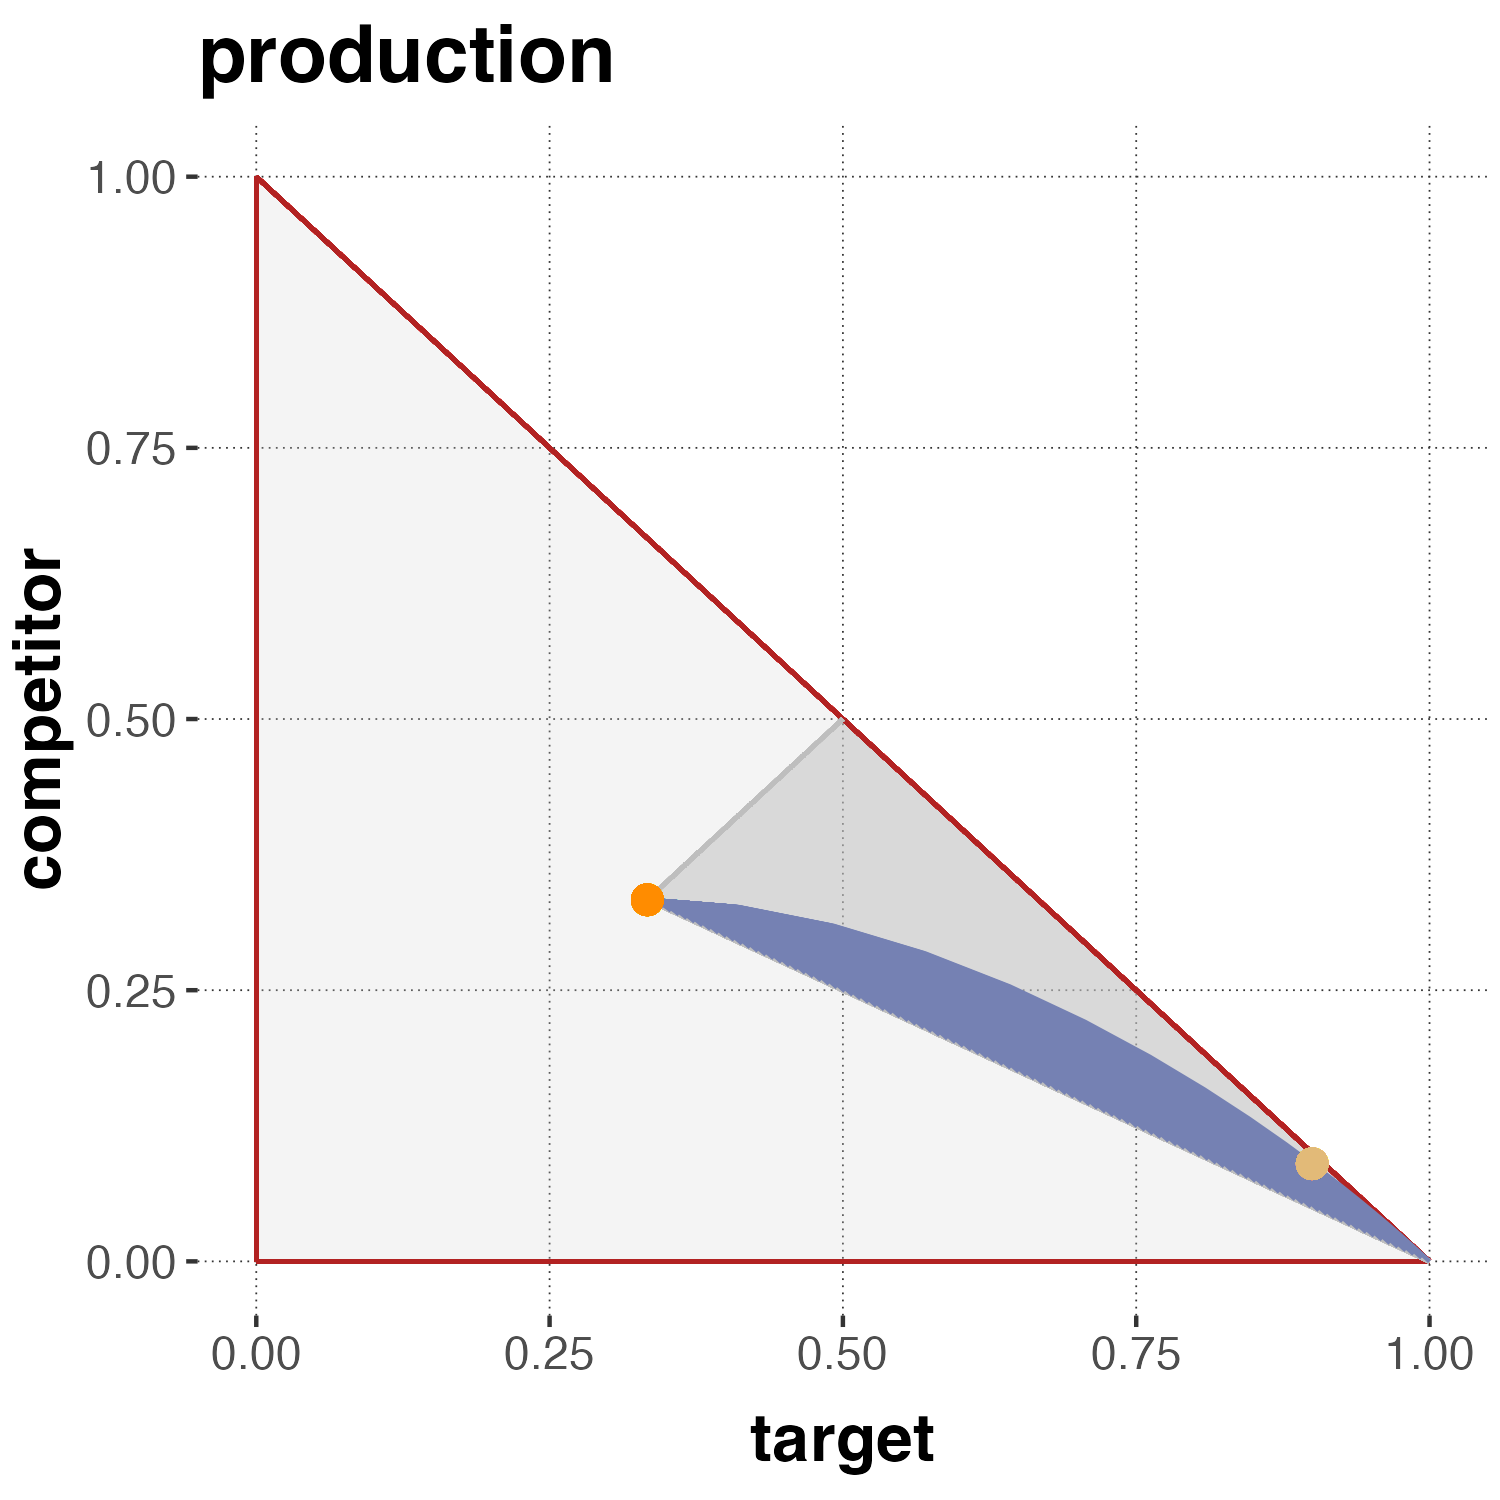
\includegraphics[width=0.45\textwidth]{00-pics/prediction-range-prod.png}
  %
  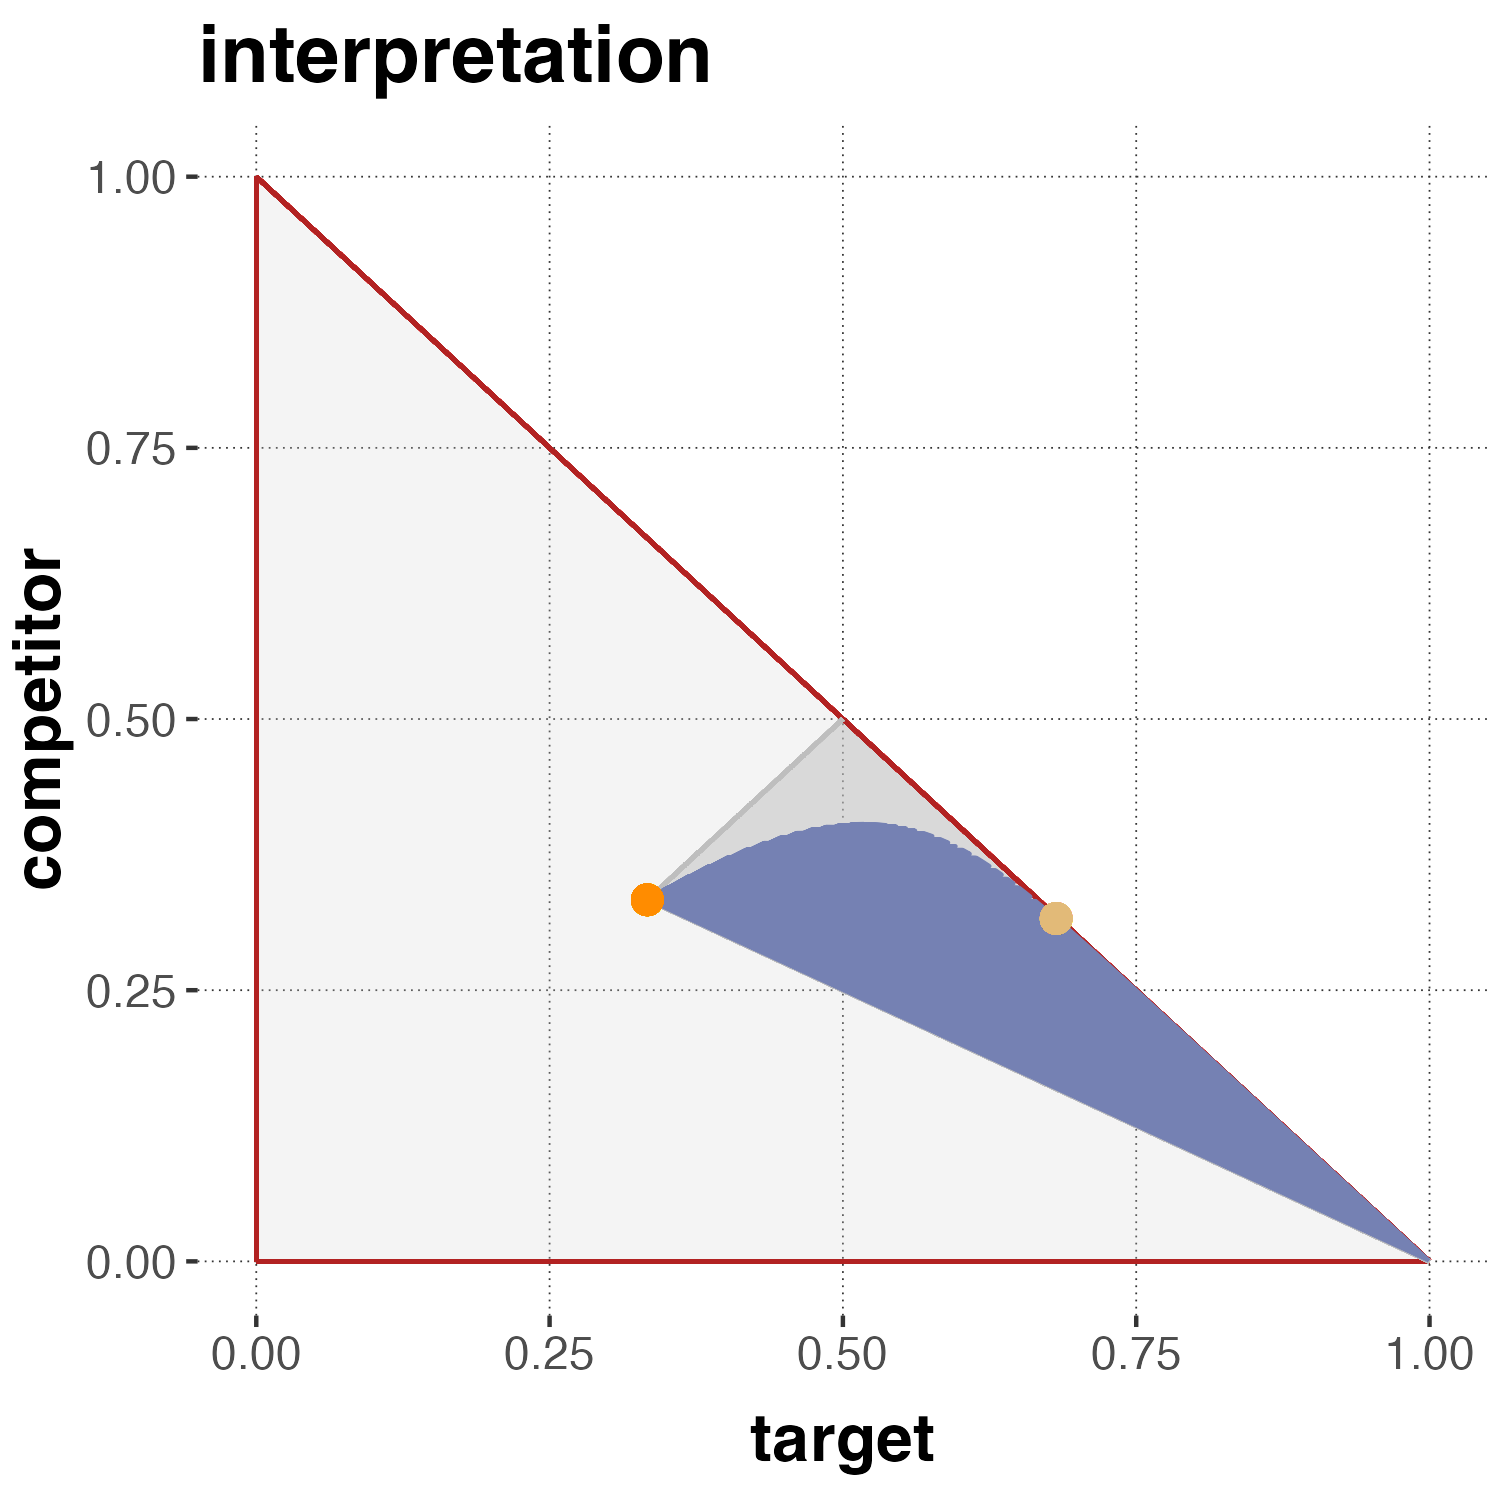
\includegraphics[width=0.45\textwidth]{00-pics/prediction-range-inter.png}

  \caption{
    Range of predictions the intermediate-scope model makes for any pair of parameter values $\alpha_{c}$ and $\epsilon_{c}$.
    The light gray triangle with the red boundary is the probability simplex, i.e., the space of all possible 3-place probability vectors.
    The darker gray area in gray boundary lines is the subspace that is compatible with the ordering that the probability of choosing the target is bigger than that of the competitor, which in turn is bigger than that of the distractor.
    The blue area is the subspace of probabilistic predictions the intermediate-scope model makes under any value of its parameters.
    The orange dot in the middle is the ``Laplace point'' of equal probability for all three options, which the model predicts for $\alpha=0$ or $\epsilon=1$.
    The yellow dot is the ``vanilla prediction'' for $\alpha_{c}=1$ and $\epsilon_{c}=0$.
  }
  \label{fig:prediction-range}
\end{figure}

\printbibliography[heading=bibintoc]

\newpage

\section*{Snippets}

\begin{itemize}
  \item for conclusion?
  \begin{itemize}
    \item The question after the human-likeness of quantitative LLM-derived information matters for applications which use numerical scores to rank or weigh options \citep[e.g.,][]{ParkOBrien2023:Generative-Agen,ZhangLehman2023:OMNI:-Open-ende}.
    Moreover, to the extent that LLMs are used as part of explanatory ``neuro-symbolic models'' of information processing \citep{GarcezLamb2020:Neurosymbolic-A}, understanding whether and how LLMs might yield full-fledged distributional predictions is important, e.g., to explore their integration into probabilistic (cognitive) models \citep[c.f.,][]{Frank2023:Large-language-}.
  \end{itemize}
  \item PT: the high-level take-away that item-level LLM predictions don't fit human predictions well might, as always, be met with the comment that the task is rather artificial. maybe this should go into the discussion
  \item FC: The fact that the aggregate predictions track aggregate human behaviour means that the discrepancies are washing out. But there's also the interesting question of finding the systematic differences between LLMs and people. The task then would be to find sets of stimuli where the differences do \emph{not} wash out and ask: What if anything do these stimuli share? This paper could also be a jumping board for this line of research.
  \item PT: maybe a conclusion in the spirit of "cogmod in the age of LLMs"/ "computational psycholinguistics \& careful assessment of reasoning / linguistic abilities of LLMs against human performance" might be not entirely ludicrous too
\end{itemize}



\end{document}
